\documentclass[british,titlepage]{ntnuthesis}

\title{An NTNU Thesis \LaTeX{} Document Class}
\shorttitle{An NTNU Thesis Document Class}
\author{Community of Practice in Computer Science Education at NTNU}
\shortauthor{CoPCSE$@$NTNU}
\date{CC-BY \ntnuthesisdate}

\addbibresource{thesis.bib}

\usepackage{tikz}
\usetikzlibrary{bayesnet}
\usepackage{ifthen}


% From https://www.overleaf.com/learn/latex/Glossaries

\makeglossaries % Prepare for adding glossary entries



% --------------------
% ----- Acronyms -----
% --------------------

\newacronym{gp}{GP}{Gaussian Process}
\newacronym{mcmc}{MCMC}{Markov Chain Monte Carlo}
\newacronym{pgm}{PGM}{Probabilistic Graphical Model}
\newacronym{bp}{BP}{Belief Propagation}
\newacronym{dgm}{DGM}{Directed Graphical Model}
\newacronym{bn}{BN}{Bayesian Network}
\newacronym{mrf}{MRF}{Markov Random Field}
\newacronym{kl}{KL}{Kullback-Liebler divergence}
\newacronym{pdf}{PDF}{Probability Density Function}
\newacronym{pmf}{PMF}{Probability Mass Function}
\newacronym{vi}{VI}{Variational Inference}
\newacronym{elbo}{ELBO}{Evidence Lower Bound}
\newacronym{hmc}{HMC}{Hamiltonian Monte Carlo}
\newacronym{nuts}{NUTS}{No-U-Turn sampler}
\newacronym{colav}{COLAV}{Collision Avoidance}
\newacronym{ml}{ML}{Machine Learning}
\newacronym{sog}{SOG}{Speed Over Ground}
\newacronym{cog}{COG}{Course Over Ground}
\newacronym{rbf}{RBF}{Radial Basis Function}

\newglossaryentry{moralization}
{
    name=moralization,
    description={The process of converting Directed Graphical Models into Markov Random Fields}
}

\newglossaryentry{support}{
    name=support,
    description={The set of possible outcomes/values with a non-zero probability, i.e. all events that can happen. A Gaussian distribution for example have support for $x \in \mathcal{R}$ since it has a non-zero probability, $p(x) > 0$, for all real numbers $x \in \mathcal{R}$.}
}

\newglossaryentry{colregs}{
    name=COLREGS,
    description={International Regulations for Preventing Collisions at Sea, a set of rules for ships navigating at sea.}
} % add glossary and acronym lists before document

\begin{document}

\chapter*{Abstract}

Autonomous ships depend on situational awareness in order to avoid collisions in a safe and robust manner. By knowing the intention of surrounding vessels, safety margins can be improved by avoiding situations with increased risk. In this thesis, methods for Bayesian Inference will be explored, with the goal of developing a flexible framework for intention modelling. Exact and approximate inference methods are explored. Approximate methods are found to be more flexible, allowing easier incorporation of existing knowledge from domain experts or conventions such as \Gls{colregs}. Methods such as \acrfull{mcmc} and \acrfull{vi} are therefore explored further and compared on an illustrative intention model. The results then find \acrshort{mcmc} to be accurate at the cost of computational complexity. \acrshort{vi} on the other hand, is found to be a lot faster, though much less precise on the illustrative model. 
\chapter*{Sammendrag}



\tableofcontents
\listoffigures
\listoftables
\lstlistoflistings


\printglossary[type=\acronymtype] % Print acronyms
\printglossary                    % Print glossary

\chapter{Introduction}

Humans, while resourceful, are prone to loss of focus, tiredness and have limited attention span. Human errors are estimated to contribute to more than $75\%$ of maritime accidents \cite{Tengesdal2020RiskbasedAM}. On the contrary, computers always remain "focused" and never gets tired. Using autonomus ships in order to reduce the potential for human errors can greatly reduce the number of maritime accidents.
While completely avoiding humans at sea would increase safety, it simply is unrealistic. Autonomous ships will need cooperate with humans on nearby vessels to avoid dangerous situations. Such up-to-date situational awareness is critical to develop decision-making systems in dynamic environments \cite{endsley}. Robust \acrfull{colav} are necessary to  maneuver in areas with potential obstacles in order to avoid collisions. However, the optimal decision is usually highly situation-dependent and requires ability to understand and predict the traffic patterns of nearby vessels, either controlled by humans or autonomous. The optimal decision are further influenced by conventions such as \Gls{colregs}, especially for larger vessels. Still, some scenarios may even require rules and conventions to be broken due to unforeseen circumstances.
However, teaching machines situational awareness is not an easy task. Human's remarkable ability to recognize situations from observations is very hard to replicate in an autonomous systems.

\section{Existing research}
 Existing research on intention modelling for autonomous ships is limited. \cite{Tengesdal2020RiskbasedAM} propose a Probabilistic Scenario-Based Model Predictive Control scheme which is able to utilize probabilistic information about obstacle intentions. It demonstrates how it is possible to make safer decisions when utilizing the additional intent information. The paper propose a general framework for intention inference using \acrfull{bn}, allowing several factors to influence an obstacle's intention. However, the paper only propose an illustrative model where the parameters of the model are assumed known and do not further discuss how these models can be found or used in practice.  

Some related research has been made in the area of autonomous cars. \cite{song} explore how Hidden Markov Models (HMM) can be used to infer the intention of cars in an intersection and then utilize this information in a partially observable Markov decision process (POMDP). 


\section{Bayesian Networks}
Bayesian Networks, often called Belief Networks, are Probabilistic Graphical Models represented as directed acyclic graphs \cite{murphy}. There is strictly speaking nothing Bayesian about Bayesian Networks (they may just as well be used with Frequentist statistics), as it is simply a way to describe probability distributions. Bayesian Networks are also often used to represent causal relations, though the interactions are in no way required to be causal. However, the causal interpretation of Bayesian Networks allow humans to intuitively understand relations between variables. Bayesian Networks are for this reason heavily used in Causal Inference, which attempts to model and infer true causal relationships between variables \cite{causal}. Bayesian Networks intuitive structure further allows human domain experts to reason about and participate in the development of statistical models, without requiring deep statistical knowledge. 
This makes Bayesian Networks a good choice for intention models, as the model need to incorporate prior knowledge such as intuitive reasoning, human experts and predefined rules (such as \Gls{colregs}), as well as be able to learn from new and historical observations. 

\section{Goal}
This thesis will investigate how inference can be performed from available data in a Bayesian Network. At this point the goal is not to find a realistic intention model, but rather try to develop a flexible framework for inference in a known model. Methods which makes few assumptions about the model and makes it easy to incorporate existing knowledge will be the main focus of this thesis. This choice comes from a belief that a good intention model will need to strongly rely on prior knowledge from human experts and from predefined rules. Restricting the model by assumptions made by the inference methods, may end up restricting the ability to accurately encode such information into the model. Approximate Methods such as \acrfull{mcmc} and \acrfull{vi} will therefore be explored in greater detail, while exact methods are only presented as possible solutions for special cases where the assumptions are reasonable. The methods can in some cases be combined, by utilizing exact inference wherever the assumptions are reasonable, and fall back to approximate methods on the parts where exact methods falls short \cite{winnbishop}.
This thesis is structured into multiple chapters. Some necessary theoretical background, mainly an introduction to Bayesian Statistics and \acrfull{pgm}'s, are presented in \cref{chap:theory}. The theory for \acrshort{mcmc} based methods are then found in \cref{chap:mcmc}, while exact and approximate analytical methods are found in \cref{chap:analytical}. In order to not only present the theoretical concepts, implementations of \acrshort{mcmc} and \acrshort{vi} are compared on a fictitious model in \cref{chap:impl}. Finally, the theory and results for the different methods are then compared and discussed in \cref{chap:discussion}.
\chapter{Neccessary Theoretical Background}

\section{Useful Results From Probability Theory}

The reader is assumed to have basic understanding of probability theory. Some of the most relevant results are summarized here.
 
 \subsection{Notation}
 
 The notation $p(X)$ is used to denote the probability distribution of the random variable $X$.
 
 For \textbf{discrete} random variables the notation is straight forward. 
 \begin{align*}
 p(X) &= p(X=x)\\  &= p_X(X=x)\\ &= \Pr\{X = x\}
 \end{align*}
 
 For \textbf{continuous} random variables the probability of a single outcome is always zero, i.e. $p(X = x) \equiv 0$, as there are infinitely many possible outcomes. The notation $p(X)$ then denotes the probability density function (PDF) of $X$. 
 
 The notation $\Pr\{\cdot\}$, such as $\Pr\{X=x\}$ and $\Pr\{X \leq x\}$, is used to denote probability of a specific event occurring. The output of this operator is always a probability, i.e. $\Pr\{\cdot\} \in (0, 1)$. 
 
 
 
\subsection{Joint Probabilities}
The \textit{joint probability} $p(X, Y)$ is the probability that both $X$ and $Y$ occurs \cite[p.~29]{murphy}.

\begin{equation}
    p(X, Y) = p(X \cap Y) = p(X | Y)p(Y)
\end{equation}

\subsection{Conditional Probabilities}
The \textit{conditional probability} $p(X | Y)$ is the probability of $X$ occurring, given the known occurrence of another event $Y$. This can be interpreted as knowing the value of $Y$ includes some information about $X$. Mathematically it can be expressed as \cite[p.~29]{murphy}
\begin{equation}\label{eq:conditional_probability}
    p(X | Y) = \frac{p(X, Y)}{p(Y)}
\end{equation}

\subsection{Bayes Rule}

A useful extension to equation \eqref{eq:conditional_probability} is to recognize that the joint distribution $p(X, Y)$ can be rewritten as a product of a conditional probability $p(Y | X)$ and $p(X)$. Inserting into equation \eqref{eq:conditional_probability} yields \textit{Bayes Rule}
\begin{equation}\label{eq:bayes_law}
    p(X | Y) = \frac{p(X, Y)}{p(Y)} = \frac{p(Y | X)p(X)}{p(Y)}.
\end{equation}

As $Y$ is known, the denominator $p(Y)$ is simply a normalizing constant. It is sometimes useful to rewrite equation \eqref{eq:bayes_law} as
\begin{equation}\label{eq:bayes_law_proportional}
    p(X | Y) = \frac{p(Y | X) p(X)}{p(Y)} \propto p(Y | X)p(X)
\end{equation} 
if $p(Y)$ is hard to calculate and the normalized value of $p(X | Y)$ is not needed.

\subsection{Marginal Probability \& The Law of Total Probability}\label{sec:marginal_prob}
The \textit{marginal probability} of an event $X$ is the probability of $X$ occurring irrespective of any other variables.
For notational simplicity the integral operator is used for marginalization of both continuous and discrete random variables, even though the integral is replaced by a sum for discrete random variables. For an event $X$ and any other variables $\bf Y$, the marginal probability of $X$ can be written as
\begin{equation}
    p(X) = \int_{\boldsymbol{Y}} p(X, \boldsymbol{Y}) d\boldsymbol{Y} = \int_{\boldsymbol{Y}} p(X | \boldsymbol{Y}) p(\boldsymbol{Y}) d\boldsymbol{Y}
\end{equation}
The last equality is by the \textit{Law of total probability}, which relates marginal probabilities to conditional probabilities.

\subsection{Independence \& Conditional Independence}
If the joint probability of two variables $X$ and $Y$ can be expressed as a product of two marginals, then they are \textit{marginally independent}.
\begin{equation}
    X \perp Y \iff p(X, Y) = p(X | Y)p(Y) = p(Y | X)p(X) = p(X)p(Y)
\end{equation}

Marginal independence is rare, as most variables usually influence each other in some way. However, the variables often affect one another indirectly through other variables. The variables $X$ and $Y$ are said to be \textit{conditionally independent} given $Z$, if the conditional joint can be written as a product of conditional marginals \cite[p.~31]{murphy}:
\begin{equation}\label{eq:conditional_independence}
    X \perp Y | Z \iff p(X, Y | Z) = p(X | Z)p(Y | Z)
\end{equation}

\subsection{Interpretations of Probability}
The results mentioned so far stem from abstract mathematical axioms, and do not tell how to interpret the resulting probabilities. Different interpretations are commonly accepted. The perhaps two biggest interpretations are the Frequentist and Bayesian interpretations. 

\begin{description}
    \item[The Frequentist Interpretation:] The Frequentists define an event's probability as the limit of its relative frequency over many trials. In other words, the probabilities are assigned a physical interpretation and remains rather objective. There do however arise issues and paradoxes when assigning probabilities to events which are not recurrent, i.e. they only happen a few times. The Frequentist interpretation assumes that the collected data is random and that the model (and its corresponding parameters) are fixed. The main goal of the Frequentists are therefore to create consistent methods for dealing with uncertain data.
    \item[The Bayesian Interpretation:] The Bayesians interpret probability as a state of knowledge \cite{Jaynes86bayesianmethods:}. In Bayesian analysis the data is fixed, whereas the model is unknown. Data is used to update prior knowledge about the model, and the probabilities are used to quantify how strongly one believe in each outcome. This interpretation is highly philosophical, but beautifully captures humans' intuitive reasoning. The Bayesian interpretation does however involve a level of subjectivity when choosing priors, making it difficult to form objective opinions from data. For those interested, see \Cite{Jaynes86bayesianmethods:} for a fascinating read on the history of Bayesian probability.
\end{description}

While the differences between the Frequentist and Bayesian interpretations are mostly philosophical, there are a few practical differences. For a Frequentist it does not make sense to talk about any probabilities before an experiment has been performed. The prior $p(X)$ and posterior $p(X | Y)$ is therefore nonsensical and cannot be computed using a Frequentist interpretation.



\section{Identifiability}



\section{Bayesian Statistics}

Using \cref{eq:bayes_law} one can write 
\begin{equation}\label{eq:bayes_learning}
    p(\boldsymbol{\theta}| \mathcal{D}, \boldsymbol{\eta}) = \frac{p(\mathcal{D} | \boldsymbol{\theta}) p(\boldsymbol{\theta} | \boldsymbol{\eta})}{p(\mathcal{D})} \propto p(\mathcal{D} | \boldsymbol{\theta})p(\boldsymbol{\theta} | \boldsymbol{\eta})
\end{equation}

If $\boldsymbol{\theta}$ is the unknown parameters of a process, $\mathcal{D}$ is collected data or observations, and $\boldsymbol{\eta}$ is all prior knowledge about $\boldsymbol{\theta}$, then equation \eqref{eq:bayes_learning} is a mathematical representation of the process of learning from data \cite{Jaynes86bayesianmethods:}.

\cref{eq:bayes_learning} can be interpreted as
\begin{description}
    \item[The Prior $p(\boldsymbol{\theta} | \boldsymbol{\eta})$:] The prior incorporates knowledge about $\boldsymbol{\theta}$ before observing any data. This can be domain-specific knowledge, results from prior experiments or intuitive reasoning about possible values of $\boldsymbol{\theta}$. 
    \item[The Likelihood $p(\mathcal{D} | \boldsymbol{\theta})$]: The likelihood of the observations $\mathcal{D}$ is how well the observations fit with prior beliefs $\boldsymbol{\theta} | \boldsymbol{\eta}$. In other words, how likely it is to observe $\mathcal{D}$ if the current belief $\boldsymbol{\theta}$ were to be true.
    \item[The Posterior $p(\boldsymbol{\theta} | \mathcal{D}, \boldsymbol{\eta})$]: The posterior distribution is the updated belief about $\boldsymbol{\theta}$. This is knowledge about $\boldsymbol{\theta}$ after observing the data. 
\end{description}

The conditional variable $\boldsymbol{\eta}$ is usually omitted for simplified notation, but is implicitly defined through the choice of prior distribution, i.e. $p(\boldsymbol{\theta}) = p(\boldsymbol{\theta} | \boldsymbol{\eta})$


\subsection{Choice of prior}

\begin{description}
\item[The Bayesian Approach:]As the prior $\boldsymbol{\eta}$ can be hard to determine, the Bayesian approach is to define priors on priors. This is called a hierarchical Bayesian model and allows for complex models with multiple dependent variables affecting each other through priors \cite{murphy}. The relation between the variables can be represented as a graphical model:

\begin{figure*}[h!]
\centering    
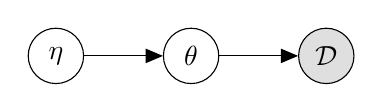
\begin{tikzpicture}
    \node[latent] (e) {$\boldsymbol{\eta}$};
    \node[latent, right=of e] (t) {$\boldsymbol{\theta}$};
    \node[obs, right=of t] (d) {$\mathcal{D}$};
    \edge {e} {t}
    \edge{t} {d}
\end{tikzpicture}
\end{figure*}

\item[Uninformative Priors:] An uninformative prior is a distribution which does not favor any outcome, and thereby does not incorporate any prior knowledge. It is like saying one simply does not know what to believe.
\item[Empirical Bayes:] The priors can be estimated from the data, resulting in the so-called Empirical Bayes method. The parameters of the prior can be found by maximizing the conditional likelihood. %TODO: cite
\end{description}


\section{Stochastic Modelling}

\subsection{Markov Chains}
A Markov Chain is a chain of events, where the outcome of the next event only depends on the current state. All information needed to predict the future is contained in the current state. This property is called the \textit{Markov Property} and is expressed in \cref{eq:theory_markov_property}.

\begin{equation}\label{eq:theory_markov_property}
p(\mathbf{X}_{t+1} | \mathbf{X}_t,  \mathbf{X}_{0:t-1}) = p(\mathbf{X}_{t+1} | \mathbf{X}_t)  \quad \forall t \in [1, \infty)
\end{equation}

\subsubsection{Stationary Distribution}
As time moves on, some states will be visited more frequently than others. This long-running distribution of states is called the \textit{stationary distribution} of the Markov Chain. If $\mathbf{P}$ is the transition probability matrix for a discrete Markov chain, then $\boldsymbol{\pi}$ is the stationary distribution if 
\begin{equation}\label{eq:markov_stationary}
    \boldsymbol{\pi} = \boldsymbol{\pi} \mathbf{P}
\end{equation}

The stationary distribution may not be unique, and whether a unique stationary distribution exists, depends on how the Markov Chain behaves. Further details on stationary distributions are outside the scope of this thesis. 



\section{Probabilistic Graphical Models}
\textit{\acrfull{pgm}}, often called Bayesian Networks, allows for efficient factorization of the joint distribution by assuming conditional independence, as defined in \cref{eq:conditional_independence}, between variables. \acrshort{pgm}'s are graphs, where nodes represent random variables and edges represents statistical dependence between the variables. By utilizing the independence assumptions in the graphs, the computational complexity can be drastically reduced \cite{murphy}.

\subsection{\acrfull{dgm}}
\acrshort{dgm}'s are perhaps the simplest type of \acrshort{pgm} and is based on \textbf{Directed Acyclic Graphs} (DAG). It is a graph structure which do not allow cycles and all edges are directed. The flow of information is explicitly modeled in the direction on the edges. \acrshort{dgm}'s are well-suited for modelling causal relationships and when the flow of information is clearly directed. An example can be the relationship between the state of a physical system and a sensor. The system affects the sensor, but the sensor does not affect the system. For the \acrshort{dgm} in \cref{fig:dgm}, the variables $B$ and $C$ are conditionally independent given $A$, i.e. $B \perp C | \; A$. However, knowing $D$ restricts $C$ and $B$, i.e. $B \not\perp C | \; D$. This all comes directly from inspecting the graph. 

\acrshort{dgm} allows for straight-forward factorization of the joint-distribution 
\begin{equation}\label{eq:dgm_factorization}
    p(\mathbf{x}) = \prod_{v \in \mathcal{V}}p(v | \mathbf{pa}(v))
\end{equation}
where $\mathcal{V}$ is all the nodes in the graph and $\mathbf{pa}(v)$ is the parent's for node $v$. 

\subsection{\acrfull{mrf}} \label{sec:mrf}

\acrshort{mrf}'s are undirected graphical models, and offers a more general specification of independence assumptions. They are in some domains, such as relational or spatial data , more natural than \acrshort{dgm}'s as they are symmetric, i.e. the information flows both ways \cite{murphy}. The \acrshort{mrf} in \cref{fig:mrf} shows that $B$ and $C$ is only independent if both $A$ and $D$ is observed, i.e. $B \perp C | \; A, D$. The important thing to notice is that the \acrshort{mrf} makes vastly different assumptions than the \acrshort{dgm}, even though the structure is similar.

By the \textbf{Hammersley-Clifford Theorem} \cite[p.~ 668]{murphy}, the joint distribution of \acrshort{mrf} models can be factorized on the form
\begin{equation}
    p(\mathbf{x}) =\frac{1}{Z} \prod_{c \in \mathcal{C}} \psi_c(\mathbf{x}_c)
\end{equation}
where is $\mathcal{C}$ is the set of all \textit{maximal cliques}, i.e. largest, fully connected sub graphs. All variables in a maximal clique is therefore dependent on each other. $\psi_c(\cdot)$ is the \textit{(factor) potential function} for the nodes in the clique $c$, and determines the strength of the interaction between the variables $\bf{x}_c$. The \textit{(factor) partition function}
\begin{equation}
    Z = \int_\mathbf{x} (\prod_{c \in \mathcal{C}} \psi_c(\mathbf{x}_c)) d \mathbf{x}
\end{equation}
is a normalization constant so that $p(\mathbf{x}) \in [0, 1]$. The potential functions $\psi_c(\cdot)$ can therefore be arbitrary non-negative functions. 

\acrshort{dgm}'s can be converted into \acrshort{mrf}'s through \textit{\gls{moralization}}. \Gls{moralization} is performed by making all edges undirected and add new edges between variables sharing a child. Some independence information is lost in the process, but it represent the same factorization of the joint distribution. The computational complexity of inference on \acrshort{dgm}s and \acrshort{mrf}s are, generally speaking, the same  \cite{murphy}. Inference methods for \acrshort{mrf}'s can therefore also be used on \acrshort{dgm}'s by first moralizing.


\subsection{Factor Graphs}
Factor Graphs unifies the concept of directed (\acrshort{dgm}) and undirected graphical models (\acrshort{mrf}). A factor graph is an undirected bipartite graph. Bipartite graphs are graphs with two different types of nodes, factors and variables. All variables are represented by round nodes and all factors are square nodes. Each factor is connected to all variables it references through undirected edges. Both \acrshort{mrf}'s and \acrshort{dgm}'s can be converted to factor graphs. Factor graphs is not really intended for modelling independence, but rather visualize how the joint distribution can be factorized to allow for efficient computations. \cref{fig:factor} shows a factor graph for the \acrshort{mrf} in \cref{fig:mrf}.

For generative models, an extension to factor graph notation is proposed in \cite{dietz} to allow for a more intuitive reasoning about the model. The directed edges in \cref{fig:factor_directed} contains additional information about how realizations of the random variables are generated, similar to the \acrshort{dgm} in \cref{fig:dgm}. The factors can the be viewed intuitively as generative processes, with input and output variables. It otherwise contain the exact same functional representation as the normal factor graph in \cref{fig:factor}. 

\begin{figure}[h]
\centering
\begin{subfigure}{0.49\textwidth}
\centering
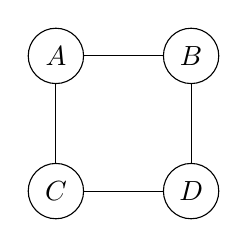
\begin{tikzpicture}
    \node[latent] (A) {$A$};
    \node[latent, right=of A] (B) {$B$};
    \node[latent, below=of A] (C) {$C$};
    \node[latent, below=of B] (D) {$D$};
    \edge[-] {A} {B};
    \edge[-] {A} {C};
    \edge[-] {C} {D}
    \edge[-] {B} {D}
\end{tikzpicture}
\caption{\acrfull{mrf}}
\label{fig:mrf}
\end{subfigure}
\begin{subfigure}{0.49\textwidth}
\centering
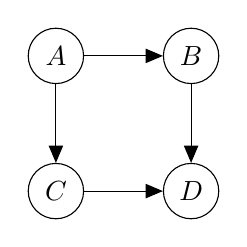
\begin{tikzpicture}
    \node[latent] (A) {$A$};
    \node[latent, right=of A] (B) {$B$};
    \node[latent, below=of A] (C) {$C$};
    \node[latent, below=of B] (D) {$D$};
    \edge {A} {B};
    \edge {A} {C};
    \edge {C} {D}
    \edge {B} {D}
\end{tikzpicture}
\caption{\acrfull{dgm}}
\label{fig:dgm}
\end{subfigure}
\begin{subfigure}{0.49\textwidth}
\centering
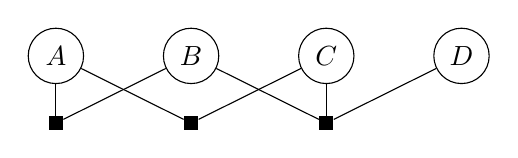
\begin{tikzpicture}
    \node[latent] (A) {$A$};
    \node[latent, right=of A] (B) {$B$};
    \node[latent, right=of B] (C) {$C$};
    \node[latent, right=of C] (D) {$D$};
    \factor[below=of A] {ba-factor} {} {} {};
    \factor[below=of B] {ca-factor} {} {} {};
    \factor[below=of C] {dbc-factor} {} {} {};
    \factoredge{A, B}{ba-factor}{}
    \factoredge{A, C}{ca-factor}{}
    \factoredge{B, C, D}{dbc-factor}{}
\end{tikzpicture}
\caption{Factor Graph}
\label{fig:factor}
\end{subfigure}
\begin{subfigure}{0.49\textwidth}
\centering
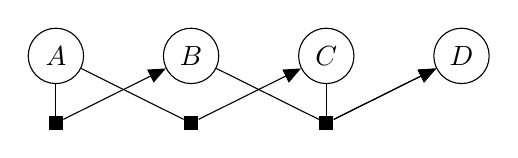
\begin{tikzpicture}
    \node[latent] (A) {$A$};
    \node[latent, right=of A] (B) {$B$};
    \node[latent, right=of B] (C) {$C$};
    \node[latent, right=of C] (D) {$D$};
    \factor[below=of A] {ba-factor} {} {} {};
    \factor[below=of B] {ca-factor} {} {} {};
    \factor[below=of C] {dbc-factor} {} {} {};
    \factoredge{A}{ba-factor}{B}
    \factoredge{A}{ca-factor}{C}
    \factoredge{B}{dbc-factor}{D}
    \factoredge{C}{dbc-factor}{D}
\end{tikzpicture}
\caption{Factor Graph for generative model}
\label{fig:factor_directed}
\end{subfigure}

\caption{\acrshort{pgm} representations of a probabilistic models with $4$ variables.}
\end{figure}

\section{Probability Distributions}

\subsection{Transformations}
TODO: Add equation

\subsection{Conjugate Priors}\label{sec:theory_conjugate_priors}
If the posterior distribution is in the same family as the prior, then the posterior is called the \textit{conjugate distribution} and the prior is called the \textit{conjugate prior}. Using conjugate priors in Bayesian Statistics, allows for analytically tractable inference as the posterior becomes a well known probability distribution. \cref{table:conjugate_priors} summarizes the conjugate priors for a few common distribution.


\begin{table}[h]
\begin{tabular}{lllll}
\hline
\multicolumn{1}{|l|}{\textbf{Distribution}} & \multicolumn{1}{l|}{\textbf{1st Parent}}        & \multicolumn{1}{l|}{\textbf{Conjugate}} & \multicolumn{1}{l|}{\textbf{2nd Parent}} & \multicolumn{1}{l|}{\textbf{Conjugate}} \\ \hline
\multicolumn{1}{|l|}{Gaussian}              & \multicolumn{1}{l|}{mean $\mu$}                 & \multicolumn{1}{l|}{Gaussian}           & \multicolumn{1}{l|}{precision $\gamma$}  & \multicolumn{1}{l|}{Gamma}              \\ \hline
\multicolumn{1}{|l|}{Gamma}                 & \multicolumn{1}{l|}{shape $\alpha$}             & \multicolumn{1}{l|}{none}               & \multicolumn{1}{l|}{scale $b$}           & \multicolumn{1}{l|}{Gamma}              \\ \hline
\multicolumn{1}{|l|}{Discrete}              & \multicolumn{1}{l|}{probabilities $\mathbf{p}$} & \multicolumn{1}{l|}{Dirichlet}          & \multicolumn{1}{l|}{parents $\{x_i\}$}   & \multicolumn{1}{l|}{Discrete}           \\ \hline
\multicolumn{1}{|l|}{Dirichlet}             & \multicolumn{1}{l|}{pseudo-counts $\bf a$}      & \multicolumn{1}{l|}{none}               & \multicolumn{1}{l|}{}                    & \multicolumn{1}{l|}{}                   \\ \hline
\multicolumn{1}{|l|}{Exponential}           & \multicolumn{1}{l|}{scale $\alpha$}             & \multicolumn{1}{l|}{Gamma}              & \multicolumn{1}{l|}{}                    & \multicolumn{1}{l|}{}                   \\ \hline
\multicolumn{1}{|l|}{Poisson}               & \multicolumn{1}{l|}{mean $\lambda$}             & \multicolumn{1}{l|}{Gamma}              & \multicolumn{1}{l|}{}                    & \multicolumn{1}{l|}{}                   \\ \hline
\end{tabular}
\caption{Table of conjugate priors for common, standard distributions. For cells with \textit{none}, there exist no standard distribution as a conjugate prior. \cite[p.~676]{winnbishop}}
\label{table:conjugate_priors}
\end{table}


\subsection{Beta \& Dirichlet Distributions}
The Beta distribution is a distribution with support between $0$ and $1$, and is therefore well suited to model probabilities. The Dirichlet distribution is a multivariate generalization of the Beta distribution. 
\subsection{Binomial \& Multinomial Distributions}
\subsection{Dirichlet-Multinomial Distribution}
\subsection{Bernouilli \& Categorial Distributions}
\subsection{Normal Distribution}
\subsection{The Exponential Family}
The Exponential Family is a family of distribution for which the \acrshort{pdf} or \acrshort{pmf} can be expressed on the from
\begin{equation}
    p(\mathbf{x} | \boldsymbol{\theta}) = h(\mathbf{x}) \exp[\eta(\boldsymbol{\theta}) T(\mathbf{x}) - A(\boldsymbol{\theta})]
\end{equation}
All the distributions mentioned so far are part of the Exponential Family. Distributions in the exponential family always have conjugate priors, however they may not be standard, well-known distributions. %TODO CITE


\chapter{Monte Carlo Sampling}\label{chap:mcmc}
\section{Importance Sampling}\label{sec:theory_importance_sampling}

\section{Markov-Chain-Monte-Carlo}
The main idea behind \acrfull{mcmc} algorithms is to construct Markov Chains whose stationary distribution is the desired target density. After drawing many correlated samples from such a chain, the fraction of time spent in each state will be proportional to the target density $p^*(\mathbf{x})$ \cite{murphy}. 

\subsection{Metropolis Hastings Algorithm}
The Metropolis Hastings Algorithm (MH) is described in \cite[p.~850]{murphy}.
For each current state $\mathbf{x}$, a new state $\mathbf{x'}$ is proposed according to a proposal density $q(\mathbf{x'} | \mathbf{x})$. The proposal density can be chosen freely as long as it gives a non-zero probability of moving to states with non-zero probability in the target density. In other words, $q(\cdot)$ must cover all possible realizations of $p^*(\cdot)$. 

After proposing a move to $\mathbf{x'}$, the proposal is either \textbf{rejected} or \textbf{accepted} according to a formula which ensures that the stationary distribution of the Markov chain equals the target distribution. 

For a \textbf{symmetric} proposal distribution, i.e. $q(\mathbf{x'} | \mathbf{x}) = q(\mathbf{x}| \mathbf{x'})$, the acceptable probability is given by 
\begin{equation}
    r = \min(1, \frac{p^*(\mathbf{x'})}{p^*(\mathbf{x})})
\end{equation}

For an \textbf{asymmetric} proposal, i.e. $q(\mathbf{x'} | \mathbf{x}) \neq q(\mathbf{x} | \mathbf{x'})$, the \textit{Hastings correction} is needed to compensate for any bias introduced by $q(\cdot)$
\begin{subequations}.
\begin{align}
    r &= \min(1, \alpha)\\
    \alpha &= \frac{p^*(\mathbf{x'}) q(\mathbf{x'} | \mathbf{x})}{p^*(\mathbf{x}) q(\mathbf{x}| \mathbf{x'})}\label{eq:mcmc_mh_acceptance}
\end{align}
\end{subequations}

The normalization constant in the target density $p^*(\cdot)$ will cancel in equation \eqref{eq:mcmc_mh_acceptance}. The MH algorithm can therefore be used with unnormalized distributions, making it a very useful algorithm for sampling from complex distributions. 

The MH algorithm is summarized in \cref{alg:metropolis_hastings}.
\begin{algorithm}
\SetAlgoLined
\For(){t = 0, 1, 2}{
    Sample $x' \sim q(x' | x_t)$ \;
    Compute acceptance probability \\
    $\alpha = \frac{p^*(\mathbf{x'}) q(\mathbf{x'} | \mathbf{x}_t)}{p^*(\mathbf{x}_t) q(\mathbf{x}_t | \mathbf{x'})}$\;
    Compute $r = \min(1, \alpha)$\;
    Sample $u \sim \mathcal{U}(0, 1)$\;
    Set $x_{t+1} = \begin{cases}x' & \text{if } u \leq r\\x_t & \text{otherwise}\end{cases}$;
}
\caption{Metropolis Hastings}
\label{alg:metropolis_hastings}
\end{algorithm}

\subsection{Random Walk Metropolis}\label{sec:random_walk_metropolis}
A common proposal density is a symmetric Gaussian distribution centered at the current state, i.e. $$q(\mathbf{x'} | \mathbf{x}) = \mathcal{N}(\mathbf{x'} | \mathbf{x}, \boldsymbol{\Sigma})$$ resulting in the \textit{Random Walk Metropolis Algorithm}.

\subsection{Independence Sampling}
If the proposal density $q(\cdot)$ is independent of the current state, i.e. $$q(\mathbf{x'} | \mathbf{x}) = q(\mathbf{x'})$$ then the MH algorithm boils down to the \textit{independence sampler}, which is similar to importance sampling as described in \cref{sec:theory_importance_sampling} \cite{murphy}.

\subsection{Hamiltonian MCMC}

Sampling in a continuous state-space using \cref{alg:metropolis_hastings} with a simple proposal distribution can be slow. If the gradients of the (unnormalized) target distribution is known, other methods such as \textit{\acrfull{hmc}} can be used to drastically speed up the sampling process by proposing new states with increased likelihood of acceptance. In addition to the model parameters $\mathbf{q}$, auxiliary momentum variables $\bf p$ are sampled and used to simulate the state as a particle moving around in space. The Hamiltonian Dynamics in \cref{eq:hamiltonian_dynamics} are simulated and used to propose new states with high acceptance probability \cite{neal2012mcmc,murphy,hoffman2011nouturn,robert2018accelerating}. \acrshort{hmc} requires a few parameters to be specified. The number of \textit{leapfrog step} describes how many steps should be simulated for each proposal, while the \textit{step size} is the size of the discretization used when simulating the Hamiltonian Dynamics. Especially the number of leapfrog step can be difficult to tune, as too many leads to unnecessary computations while too few leads to random walk behaviour \cite{hoffman2011nouturn}. 

Hamilton's equations is given by \cref{eq:hamiltonian_dynamics}. $H$ is the Hamiltonian representing the total energy of the system as a function of position and momentum, usually in the form of the potential energy $U(\mathbf{q})$ and the kinetic energy as expressed in \cref{eq:hamiltonian}. In \acrshort{hmc} the potential energy $U(\mathbf{q})$ is selected to be the negative log likelihood of the (unnormalized) target distribution and $M$ is a positive definite mass matrix, typically diagonal or a scalar multiple of the identity matrix \cite{neal2012mcmc}. 
\begin{align}\label{eq:hamiltonian_dynamics}
    \frac{d q_i}{d\tau} &= \frac{\partial H(\mathbf{q}, \mathbf{p})}{\partial p_i} & \frac{d p_i}{d\tau} &= -\frac{\partial H(\mathbf{q}, \mathbf{p})}{\partial q_i}
\end{align}

\begin{align}\label{eq:hamiltonian}
    H(\mathbf{q}, \mathbf{p}) &= U(\mathbf{q}) + \frac{1}{2} \mathbf{p}^\intercal M^{-1} \mathbf{p} & U(\mathbf{q}) = - \ln p^*(\mathbf{q})
\end{align}

An extension to \acrshort{hmc}, the \textit{\acrfull{nuts}} is proposed in \cite{hoffman2011nouturn}. It eliminates the need for manual tuning of leapfrog steps and it is shown empirically to perform comparably to well tuned \acrshort{hmc} method without any manual intervention \cite{hoffman2011nouturn}.



\subsection{Burn-in}
The samples from the Markov Chain are not from the target distribution until the chain reaches its stationary distribution. A (potentially large) number of samples on the beginning of the chain are therefore invalid and are usually discarded. This is called the \textit{burn-in phase} and is one of the major weaknesses of \acrshort{mcmc} \cite{murphy}. Convergence of a Markov Chain is difficult to detect and in practice a fixed, large number of samples are discarded.   

It can be shown that if the stationary distribution of a Markov Chain exists, it will be independent of starting state \cite{murphy}. Initializing the chain at different points will not affect the stationary distribution and convergence can be verified by comparing independently sampled chains, initialized with different values. If all chains have converged toward the same value, the burn-in phase is complete.    
%TODO Add trace plot

\subsection{MCMC in practice}
Many software packages are available for \acrshort{mcmc}, such as: 

\begin{enumerate}
    \item Tensorflow Probability \cite{tensorflow2015-whitepaper}
    \item STAN \cite{stan}
    \item PyMC3 \cite{pymc3}
\end{enumerate}

In practice, these packages can handle much of the complexity performing MCMC based inference, leaving only the model specification and a few parameters to the user. These packages also handles implementation details such as efficient utilization of available hardware (GPU and CPU) and automatic differentiation. Accelerated sampling methods such as \acrshort{hmc} and \acrshort{nuts} are also easy to use in these software packages.   

\subsection{Thinning}
As new states are proposed from previous states, the samples are naturally highly auto-correlated. This results in a lot of samples which provide little additional information about the true distribution. A simple method to reduce the auto-correlation and thereby improve the information the samples is to use \textit{thinning}, were only every nth sample are kept. This can save a lot of storage \cite{murphy}.

\subsection{Convergence Guarantees}

\subsection{Bijectors}
Sampling from a constrained distribution (i.e. a Beta distribution which only offer support on $x \in (0, 1)$) using an unconstrained proposal distribution can quickly take a long time as many of the proposal will be rejected. A solution to this problem is to transform the proposal distribution such that the MCMC algorithm can sample in an unconstrained space \cite{Parno_2018, tensorflow2015-whitepaper}. 

The framework \textit{Tensorflow Probability} introduce the concept of \textit{Bijectors} which are predefined (potentially non-linear) transformations of distributions. Softmax, Softplus, Sigmoid, Affine and Exponential are among many supported transformations. Using Bijectors, the proposal distributions in Tensorflow Probability can easily be transformed into a unconstrained space without dealing with any error-prone calculations \cite{tensorflow2015-whitepaper}. 



\chapter{Analytical Methods \& Variational Inference}
For some \acrshort{pgm}'s the joint distribution may have a functional form which allow marginalization using analytical methods, i.e. directly evaluating the integrals and sums. When applicable, analytical methods allow for exact inference and avoid the randomness introduced by sampling methods. %TODO Cite or explain further 


\section{Belief Propagation}
%TODO Better citations
The computational complexity of marginalizing over many variables in a \acrshort{pgm} may be large as the number of possible hypotheses quickly increases with the number of variables. Finding the solution in a reasonable amount of time requires a strategy which avoids unnecessary computations and efficiently utilize the structure of the \acrshort{pgm}. 

\textit{\acrfull{bp}}, also called the sum-product algorithm, is an algorithm for efficient marginalization in \acrshort{pgm}'s. The algorithm utilizes dynamic programming to avoid repeating costly calculations. The method is described in detail in \cite[p .~710]{murphy}, but is summarized here with a few notational modifications. 


\subsection{Belief Propagation for trees}
To compute the marginal density for a node $r$ in a tree-structured \acrshort{pgm}, one can imagine "picking up" the tree by $r$. The remaining nodes will be pulled down by gravity and $r$ will become the root node. \acrshort{bp} will collect evidence from the leaf nodes and work its way upward toward the root, collecting evidence and marginalizing on the way. One can imagine each node computes \textbf{messages} describing the belief about their parent nodes, and passing those messages to the parent nodes \cite{murphy}.
\subsection{Message passing}
A node $t$ computes a message containing the current belief about its parent given all evidence collected at or below node $t$ \cite{murphy}. Assuming all nodes below $t$ have already calculated their messages, the belief for node $t$ becomes
\begin{equation}\label{eq:bp_belief}
    bel_t^-(x_t) \triangleq p(x_t | \mathbf{v}_t^-) = \frac{1}{Z_t}\psi_t(x_t) \prod_{c \in ch(t)} m_{c\to t}^-(x_t)
\end{equation}
where $\mathbf{v}_t^-$ is all evidence at or below node $t$, $\psi_t(x_t)$ is the local evidence at node $t$, $m_{c \to t}^-$ is the messages passed from $t$'s children, $ch(t)$ is the children nodes for node $t$ and $Z_t$ is the normalization constant for node $t$.
Assuming the belief $bel_s^-(x_s)$ for a children $s$ of node $t$ has already been calculated using \cref{eq:bp_belief},  the message $m_{s\to t}^-$ can then be computed using
\begin{equation}\label{eq:bp_message}
    m_{s \to t}^-(x_t) = \int_{x_s} \psi_{st}(x_s, x_t) bel_s^-(x_s) dx_s
\end{equation}
where $\psi_{st}(x_s, x_t)$ is the edge potential. The edge potential $\psi_{st}(x_s, x_t)$ and local evidence $\psi_t(x_t)$ here corresponds to the factor potentials discussed in \cref{sec:mrf}.

The messages and belief state for each node can then be recursively computed using \cref{eq:bp_belief} and \cref{eq:bp_message}.

\begin{subequations}
\begin{align}
p(x_r) &= \idotsint_V p(x_r, x_1,\dots,x_k) \,dx_1 \dots dx_k\\
&= \idotsint_V p(x_r | x_1)p(x_1|x_2)\dots p(x_{k-1} | x_k)p(x_k) \, dx_1 \dots dx_k\\
&= \int_{x_1} p(x_r | x_1)\underbrace{\int_{x_2}p(x1 | x2) \; \;  \dots \underbrace{\int_{x_k} p(x_{k-1} | x_k)p(x_k) \, dx_1 \dots dx_k}_{m_{k\to k-1}^-(x_{k-1})}}_{m_{x_2 \to x_1}^-(x_1)}
\end{align}
\end{subequations}

Computing all messages from leaf nodes towards the top is called the \textbf{collecting evidence}-phase and yields the marginal distribution for the root node. However, the marginal distribution for all other nodes can easily be calculated by calculating messages from the root node and distribute messages downward towards the leaf nodes. This is called the \textbf{distribute evidence}-phase. 

The belief state for nodes $s$ other than the root, can in the distribute evidence-phase be updated using
\begin{equation}\label{eq:bp_belief_top_down}
    bel_s(x_s) \triangleq p(x_s | \mathbf{v}) \propto bel_s^-(x_s) \prod_{t \in pa(s)} m_{t \to s}^+(x_s)
\end{equation}
where $\mathbf{v}$ is all evidence and $m_{t \to s}^+$ are the top-down message from $t$ to $s$, which summarizes all the remaining information in the graph about node $s$. 

The top-down messages $m_{t \to s}^+$ can be computed by combining all the evidence received by $t$, except for what $s$ sent it.

\begin{subequations}
\begin{align}
    m_{t \to s}^+(x_s) &\triangleq p(x_s | \mathbf{v}_{st}^+) = \int_{x_t}\psi_{st}(x_s, x_t)\frac{bel_t(x_t)}{m_{s \to t}^-(x_t)}dx_t \label{eq:bp_belief_updating}\\
    &= \int_{x_t} \psi_{st}(x_s, x_t)\psi_t(x_t) \prod_{c \in ch(t), c \neq s} m_{c \to t}^-(x_t) \prod_{p \in pa(t)} m_{p \to t}^+(x_t) \; dx_t\label{eq:bp_sum_product}
\end{align}
\end{subequations}

\cref{eq:bp_sum_product} is found by inserting the equation for $bel_t(x_t)$, \cref{eq:bp_belief_top_down}, into \cref{eq:bp_belief_updating}, and is called the \textit{sum-product} algorithm as it multiplies all-but-one messages and marginalizes (summing) out variables. 

While \acrshort{bp} may sound complicated, one can think of this algorithm as computing the marginal distribution of $x_r$ where each sum or integral is pushed in as far as possible to simplify calculations. By beginning with the inner-most integral, the marginalization boils down to recursively computing simple integrals or sums with only a small subset of the variables. This general method is called \textit{variable elimination}\cite{murphy}. \acrshort{bp} extends this idea by also utilizing the graph structure to reduce the computational complexity. A \acrshort{pgm} with a chain structure is used as an example to show the rather simple concept behind variable elimination and \acrshort{bp}.

\subsection{Belief Propagation on arbitrary graphs}


\subsection{Limitations of analytical methods}
The methods described so far in this chapter generally applies to both discrete and continuous random variables by replacing integrals with sums for discrete variables. However, in practice, continuous random variables quickly becomes intractable unless each parent-child in the graph are conjugate priors. Assuming conjugate priors severely limits the ability to describe the data-generating process, leaving only a few types of networks feasible. Looking back at \cref{table:conjugate_priors} for common conjugate priors, only a mix of gaussians, gamma and discrete distributions allow for multiple levels in a hierarchical model. For all other distributions, one quickly ends up in a situation where no standard conjugate exist \cite{winnbishop}. 
% TODO Cite. 
\section{Variational Bayes}
\acrshort{bp} allows for exact inference of \acrshort{pgm}'s when there exists closed-form solutions of the integrals. This is however rarely the case and is only true for carefully chosen distributions. Requiring all combination of nodes to be conjugate priors (\cref{sec:theory_conjugate_priors}) can severely limit the expressibility of a \acrshort{pgm} and is not a viable solution. 

Another approach is to approximate the target distribution $p^*(\mathbf{x} | \mathbf{v})$ with a \textbf{surrogate distribution} $q(\mathbf{x})$ constructed using conjugate priors to allow for exact inference. If $p^*(\cdot)$ and $q(\cdot)$ are similar, then \acrshort{bp} can be used on $q(\cdot)$ to do approximate inference.

\subsection{Kullback-Liebler divergence}
The \textit{\acrfull{kl}}  is used as a measure of difference between two probability distributions \cite{kullback1951,murphy}.

\begin{equation}\label{eq:kl}
    \mathbb{KL}(p^* || q) = \int_\mathbf{x} p^*(\mathbf{x}) \log \frac{p^*(\mathbf{x})}{q(\mathbf{x})} d\mathbf{x} = E_{p^*} \big[ \log \frac{p^*(\mathbf{x})}{q(\mathbf{x})} \big]
\end{equation}
The \acrshort{kl} divergence boils down to the expected difference between $p^*(\cdot)$ and $q(\cdot)$ over $p^*(\cdot)$.
In this case $p^*(\cdot)$ is only assumed known up to a normalizing constant, making the expectation in \cref{eq:kl} intractable to compute. Instead, the reverse \acrshort{kl} divergence can be used as $q(\cdot)$ is assumed known.
\begin{equation}\label{eq:reverse_kl}
    \mathbb{KL}(q || p^*) = \int_\mathbf{x} q(\mathbf{x}) \log \frac{q(\mathbf{x})}{p^*(\mathbf{x})} d\mathbf{x} = E_{q} \big[ \log \frac{q(\mathbf{x})}{p^*(\mathbf{x})} \big]
\end{equation}

\subsubsection{ELBO}
In the case of variational inference, the goal is usually to find an approximation $q(\mathbf{z})$ for the posterior $p(\mathbf{z} | \mathbf{x}$.) The reverse \acrshort{kl} can then be written as.
\begin{subequations}
\begin{align}
    \mathbb{KL}(q(\mathbf{x}) || p^*(\mathbf{x} | \mathcal{D})) &= E_q\big[\log \frac{q(\mathbf{x})}{p^*(\mathbf{x} | \mathcal{D})} \big]\label{eq:elbo_kl}\\
    &= E_q\big[\log \frac{q(\mathbf{z}) p^*(\mathbf{x})}{p^*(\mathbf{z}, \mathbf{x})} \big]\\
    &= E_q\big[\log q(\mathbf{x}) \big] - E_q\big[\log p^*(\mathbf{x}, \mathcal{D})] + E_q\big[\log p^*(\mathcal{D}) \big]\\
    &= E_q\big[\log q(\mathbf{x}) \big] - E_q\big[\log p^*(\mathbf{x}, \mathcal{D})] + \log p^*(\mathcal{D})\\
    &\leq E_q\big[\log q(\mathbf{x}) \big] - E_q\big[\log p(\mathbf{x}, \mathcal{D})]\label{eq:negative_elbo}
\end{align}
\end{subequations}

As $p(\mathcal{D})$ is assumed intractable, the reverse \acrshort{kl} cannot be evaluated. However, since the surrogate density $q(\mathbf{x})$ only depend on $\mathbf{x}$, $\mathbb{KL}(q(\mathbf{x} || p^*(\mathbf{x} | \mathcal{D}))$ can still be optimized as $p(\mathcal{D})$ is constant. In other words, minimizing \cref{eq:negative_elbo} is equivalent to minimizing \cref{eq:elbo_kl}.

This problem is usually phrased as a maximization problem, and the objective function to be \textbf{maximized} is called the \textit{\acrfull{elbo}} \cite{Blei_2017}.
\begin{equation}
    \text{ELBO}(q) = E_q\big[\log p(\mathbf{x}, \mathcal{D})] - E_q\big[\log q(\mathbf{x}) \big]
\end{equation}

Variational Inference then boils down to finding the best surrogate posterior $q^*(\mathbf{x})$ which maximizes \acrshort{elbo} or minimizing \acrshort{kl} \cite{Blei_2017}.

\begin{equation}
    q^*(\mathbf{x}) = \arg \max_{q(\mathbf{x})} \text{ELBO}(q) = \arg \min_{q(\mathbf{x})} \mathbb{KL}(q(\mathbf{x}) || p^*(\mathbf{x} | \mathcal{D}))
\end{equation}



\subsection{I or M mode projection}

Forward KL is also known as \textbf{moment-projection} (M-projection)  as it will attempt to match the moments of $q(\cdot)$ with $p^*(\cdot)$. In the case of a multimodal $p^*(\cdot)$ and unimodal $q(\cdot)$, this may not be desirable as the mean is placed in between regions of high probability. Looking at \cref{eq:kl}, the KL divergence is infinite when $p(\cdot) > 0$ and $q(\cdot) = 0$. M-projection is therefore said to be \textbf{zero avoiding} as optimizing \cref{eq:kl} needs to ensure $q(\mathbf{x}) > 0$ when $p(\mathbf{x}) > 0$. M-projection therefore tends to over-estimate the support of $p^*(\cdot)$.

Reverse KL is known as \textbf{information-projection} (I-projection). As \cref{eq:reverse_kl} is infinite when $p^*(\cdot) = 0$ and $q(\cdot) > 0$, optimizing reverse KL therefore needs to ensure $q(\cdot) = 0$ when $p^*(\cdot)=0$. I-projection is therefore said to be \textbf{zero forcing} and tends to underestimate the support for $p^*(\cdot)$ \cite{murphy}. 

\subsection{Mean Field}
The simplest method for variational inference is assuming independent variables for the surrogate distribution $q(\cdot)$. 
\begin{equation}\label{eq:mean_field}
    q(\mathbf{x}) = \prod_i q_i(x_i)
\end{equation}
However, this is in many cases a very strong assumption which may lead to poor results in the case of strong interactions in the posterior distribution. An extension called \textbf{structured mean field} can in some cases be used if the posterior has a tractable substructures (i.e. sub graphs which can be described using "simple" distributions). The variables forming tractable substructures can then be combined into "mega-variables" and \cref{eq:mean_field} can be used as an approximation.   

\subsection{Variational Message Passing}
\subsection{Variational EM}



\subsection{Calculus of Variation}
\chapter{Implementation and Results}\label{chap:impl}

This chapter focuses on comparing the performance between \acrshort{mcmc} and \acrshort{vi} methods for performing inference in a \acrshort{pgm}. Each method have their strengths and weaknesses for different types of problems. As a compromise, this chapter will focus on comparing the performance of a fictitious model in order to discuss a concrete example and to show how \acrshort{mcmc} and \acrshort{vi} can be used in practice.  

\section{The model}
As the context of this paper is intention inference for autonomous ferries, it seems fit that a similar example is used. A simple intention model is therefore proposed as an example, which relates steering angle to an intention through a mixture model. 

The angle $\theta$ is defined to be the angle between the obstacle's current course and a simple predicted course given the obstacle's final destination. The vessels are required to report their final destination, but in some cases there may be user-errors where invalid destinations are transmitted to nearby vessels. If the obstacle's reported final destination is correct, $D=0$, the angle should be closely related to the obstacle's intention and can be generated from a Gaussian selected by the intention $I$ (i.e. a mixture of Gaussian's weighted by the intention probabilities). If the obstacle report an incorrect destination, $D=1$, the angle $\theta$ is independent of intention as the obstacle may he headed in a completely different direction.

This example model is intentionally not identifiable when observing only the angles $\boldsymbol{\theta}$. This example will show how the choice of priors affect the learning process, especially when parameters are not identifiable. Through the use of informative priors the model should still be able to learn what it can from available data.   

Whether or not the final destination is valid is modelled using a Bernoulli variable $D_t$ which takes the value $1$ if the destinations is \textbf{invalid}. A Beta distribution is used to model the prior probability $p_D = \Pr \{D=1\}$, i.e. the probability of the destination being invalid.  

A few modelling assumptions are made:

\begin{description}
    \item[Assumption 1] The angles $\{\theta_1, \theta_2, \dots, \theta_t\}$ are independent
    \item[Assumption 2] The ship has equal turning characteristics for port and starboard turns. The intention probabilities are from this assumed symmetrical about $\theta=0$. 
    \item[Assumption 3] Port and starboard turns are defined to be turns where $\theta \in (0, \pi)$ and $\theta \in (-\pi, 0)$ respectively.  
\end{description}

\begin{equation}
    p_D \sim \text{Beta}, \quad p_D \in (0, 1)
\end{equation}
\begin{equation}
    D_t \sim \text{Bernoulli}(p_D), \quad D_t \in \{0, 1\}
\end{equation}

The intention in a situation $I_t$ is modelled by a Categorical discrete variable where the possible realizations are shown in \cref{tbl:intentions}. The intention probabilities $\boldsymbol{\alpha}$ are distributed according to a Dirichlet distribution.

\begin{equation}
    \boldsymbol{\alpha} \sim \text{Dirichlet}, \quad \boldsymbol{\alpha} \in \{\alpha_0, \alpha_1, \alpha_2 \in (0, 1) \; | \; \sum_i \alpha_i = 1 \}
\end{equation}
\begin{equation}
    I_t \sim \text{Categorical}(\boldsymbol{\alpha}), \quad I_t \in \{0, 1, 2\}
\end{equation}

\begin{table}[h]
\centering
\begin{tabular}{|l|l|}
\hline
$I_t=0$ & The obstacle intends to keep its current course \\ \hline
$I_t=1$ & The obstacle intends a starboard turn           \\ \hline
$I_t=2$ & The obstacle intends a port-side turn            \\ \hline
\end{tabular}
\caption{Possible realizations of the intention $I_t$}
\label{tbl:intentions}
\end{table}


The mixture components for $\theta_t$ when $D_t=0$ are Gaussian Distributions. For $I=0$, the mean is zero with unknown variance. For $I \in \{1, 2\}$ the means are assumed to have equal absolute value, but opposite sign. The value for $\mu = \mu_2 = -\mu_1$ is unknown and distributed according to a Softplus (\cref{eq:softplus}) transformed Gaussian variable. Using \cref{eq:change_of_variable} for change of variable, the distribution of $\mu$ becomes 

\begin{equation}
    \mu = f(x), \quad x \sim \mathcal{N}(x) \implies p(\mu) = \mathcal{N}(f^{-1}(\mu)) \frac{1}{|f'(f^{-1}(\mu))|} 
\end{equation}

The standard deviation is assumed equal for all intentions and is distributed according to an inverse Gamma distribution. In other words, the mixture components are assumed to have the same variance and they should be symmetrical around $\theta_t=0$.
Learning the mean $\mu$ from data allows the model to adapt to different types of ships. A small fishing vessel might rapidly change course (i.e. large $\theta_t$), while a large oil-tanker has limited ability to turn due to its size (i.e. smaller $\theta_t$). 
\begin{align}
    \mu_0 &= 0 &  \mu_{2} = - \mu_{1} = \mu &\sim \text{Gaussian} & \sigma &\sim \text{Inv-Gamma}
\end{align}
When $D=0$ and $I_t=i$, the angle is distributed according to
\begin{equation}\label{eq:theta_intention_mixture}
    p(\theta_t | D=0, I_t=i) = \mathcal{N}(\mu_i, \sigma^2), \quad \theta_t \in \mathcal{R}
\end{equation}

The marginal distribution of $\theta_t$ when $D_t=0$ becomes the Gaussian mixture model in \cref{eq:angle_gauss_mixture}.

\begin{align}\label{eq:angle_gauss_mixture}
\begin{split}
    p(\theta_t | \boldsymbol{\mu}, \sigma, D=0, \boldsymbol{\alpha}) &= \sum_{i=0}^2 \Pr\{I_t=i\}\mathcal{N}(\theta_t | \mu_i, \sigma^2) \\
    &=\Pr\{I_t=0 | \alpha_0\}\mathcal{N}(\theta_t | 0, \sigma^2)\\
    &\quad+\Pr\{I_t=1 | \alpha_1\}\mathcal{N}(\theta_t | -\mu, \sigma^2)\\
    &\quad+\Pr\{I_t=2 | \alpha_2\}\mathcal{N}(\theta_t | \mu, \sigma^2)
\end{split}
\end{align}

One issue with using a Guassian distribution for angle information is that it has support on $\mathcal{R}$, while the angles $\theta$ should ideally only have support on $(-\pi, \pi)$. In practice, this may not be a big issue as long as the probability mass is mostly kept within $(-\pi, \pi)$. Another solution could be to use a nonlinear transformation to clamp $\mathcal{R}$ to $(-\pi, \pi)$. There is however a possible issue with the mean $\mu$ as it is implicitly assumed to be positive, even if the the Gaussian distribution offer support on $\mathcal{R}$. As the angle distribution is assumed symmetrical around $\theta=0$, it is possible to swap the portside and starboard turn intentions by swapping the sign of $\mu$. This will likely cause the posterior distribution to become bimodal, as the data is unable to distinguish between the two intentions.  

\cref{fig:intention_angle} shows the likelihood for different angles for the different intentions with fixed mean and variance. 

When the obstacle's target destination is invalid, $D=1$, the angle $\theta$ is distributed according to a Uniform distribution over the range $(-\pi, \pi)$ to model how the angle contains no information about the obstacle in such a case. 

\begin{equation}\label{eq:angle_uniform}
    p(\theta_t | D=1) = \text{Uniform}(-\pi, \pi)
\end{equation}

The distribution for $\theta_t$ becomes a mixture between the Gaussian Mixture in \cref{eq:angle_gauss_mixture} and the uniform distribution in  \cref{eq:angle_uniform} as expressed in \cref{eq:angle_complete_mixture} by the law of total probability.

\begin{align}\label{eq:angle_complete_mixture}
\begin{split}
     p(\theta_t | \boldsymbol{\mu}, \sigma, p_D, \boldsymbol{\alpha})
     &= \sum_D \Pr\{D_t=d | p_D\} p(\theta_t | D_t=d, \mu, \sigma, \boldsymbol{\alpha})\\
     &= \Pr\{D_t = 0 | p_D\} \underbrace{p(\theta_t | \mu, \sigma, D_t=0, \boldsymbol{\alpha})}_{\text{\cref{eq:angle_gauss_mixture}}}\\
     &+ \Pr\{D_t=1 | p_D\}\underbrace{p(\theta_t | D_t=1)}_{\text{\cref{eq:angle_uniform}}}
\end{split}
\end{align}

The data generating process for $\theta_t$ is shown in \cref{fig:example_pgm} then becomes:

\begin{enumerate}
    \item Draw priors $p_D$, $\boldsymbol{\alpha}$, $\mu$ and $\sigma$
    \item For all $t \in \{1, \dots, N \}$, draw $D_t$ and $I_t$ conditional on $p_D$ and $\boldsymbol{\alpha}$
    \item For all $t \in \{1, \dots, N\} $, if $D_t=1$, draw $\theta_t$ from Uniform distribution. If not, draw $\theta_t$ from $\mathcal{N}(\theta_t | \mu_i, \sigma)$ conditional on $I=i$, $\mu_i$ and $\sigma$. 
\end{enumerate}

\begin{figure}[h]
    \centering
    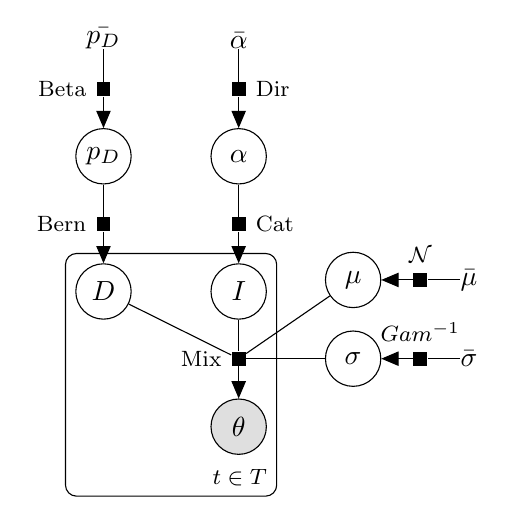
\begin{tikzpicture}
        % NODES
        \node[latent] (I) {$I$};
        \node[obs, below=of I] (theta) {$\theta$};
        \node[latent, above=of I] (alpha){$\boldsymbol{\alpha}$};
        
        % FACTORS
        \factor[below=of I] {theta-f}{left:Mix}{}{};
        \factor[above=of I]{I-f}{right:Cat}{}{};
        \factor[above=of alpha]{PI-f}{right:Dir}{}{};

        \node[latent, left= of I] (D) {$D$};
        \node[latent, above= of D] (p_D) {$p_D$};
        \node[latent, right= of theta-f, yshift=1cm] (mean) {$\mu$};
        \node[latent, right= of theta-f] (std) {$\sigma$};

        \factor[right=of mean]{mean-f}{above:$\mathcal{N}$}{}{};
        \factor[right=of std]{std-f}{above:$\text{Gam}^{-1}$}{}{};
        \factor[above=of D]{D-f}{left:Bern}{}{};
        \factor[above=of p_D]{p_D-f}{left:Beta}{}{};

        \node[const, above=of p_D] (pp_D) {$\bar{p_D}$};
        \node[const, right=of mean] (p_mean) {$\bar{\mu}$};
        \node[const, right=of std] (p_std) {$\bar{\sigma}$};
        \node[const, above=of alpha] (a) {$\bar{\boldsymbol{\alpha}}$};
        
        \factoredge {I, D, mean, std} {theta-f} {theta};
        \factoredge{alpha}{I-f}{I};
        \factoredge{a}{PI-f}{alpha};
        \factoredge{p_mean}{mean-f}{mean};
        \factoredge{p_std}{std-f}{std};
        \factoredge{pp_D}{p_D-f}{p_D};
        \factoredge{p_D}{D-f}{D};

        \plate {ship}{(I)(theta)(D)}{$t \in T$};
    \end{tikzpicture}
    \caption{\acrshort{pgm} describing the data-generating process using graphical notation. The rectangle is called a plate and express that the variables within are repeated once for each $t \in T$. The variables outside the plate are shared across all $t \in T$. The gray node for $\theta$ indicate that the variable is observed, while the rest are latent.}
    \label{fig:example_pgm}
\end{figure}



The resulting joint distribution  can then be factored into \cref{eq:example_joint}.

\begin{align}\label{eq:example_joint}
\begin{split}
    p(\boldsymbol{\theta}, \boldsymbol{\mu}, \sigma, p_D, \boldsymbol{\alpha}) =\underbrace{p(\boldsymbol{\alpha})}_{\text{Dirichlet}}\underbrace{p(p_D)}_{\text{Beta}}\underbrace{p(\mu)}_{\mathcal{N}} \underbrace{p(\sigma)}_{\text{Inv-Gamma}} \prod_t \underbrace{p(\theta_t | \mu, \sigma, p_D, \boldsymbol{\alpha})}_{\text{\cref{eq:angle_complete_mixture}}}
\end{split}
\end{align}

The unnormalized posterior distribution then becomes
\begin{align}\label{eq:example_unnormalized_posterior}
\begin{split}
    \tilde{p}(\mu, \sigma, p_D, \boldsymbol{\alpha}) =  p(\boldsymbol{\theta} = \mathcal{D}, \mu, \sigma, p_D, \boldsymbol{\alpha}) \propto p(\mu, \sigma, p_D, \boldsymbol{\alpha} | \boldsymbol{\theta}= \mathcal{D})
\end{split}
\end{align}


\begin{figure}
    \centering
    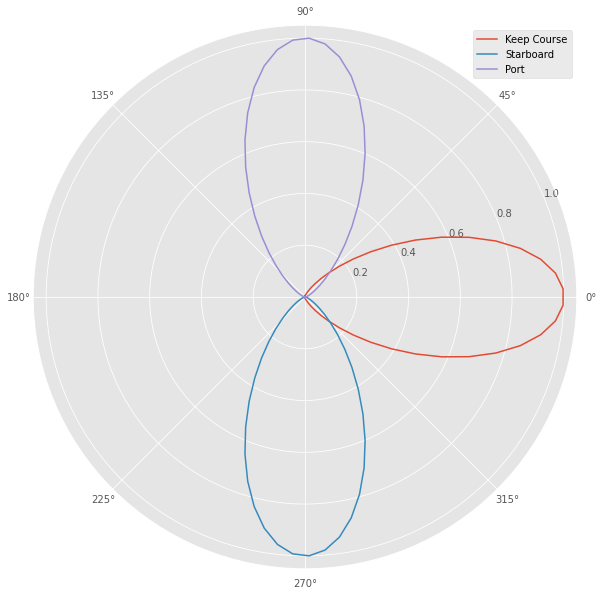
\includegraphics[width=0.7\textwidth]{figures/intention_angle.png}
    \caption{Normalized likelihood of different angles under different intention hypotheses. This is a polar plot where the angle represent $\theta_t^{(I=i)}$, the radius represent the probability. This is generated from \cref{eq:theta_intention_mixture} with $\mu_0=0$, $\mu_1 = -\frac{\pi}{2}$, $\mu_2=\frac{\pi}{2}$ and $\sigma_i=\frac{\pi}{8}$}
    \label{fig:intention_angle}
\end{figure}

\begin{figure}
    \centering
    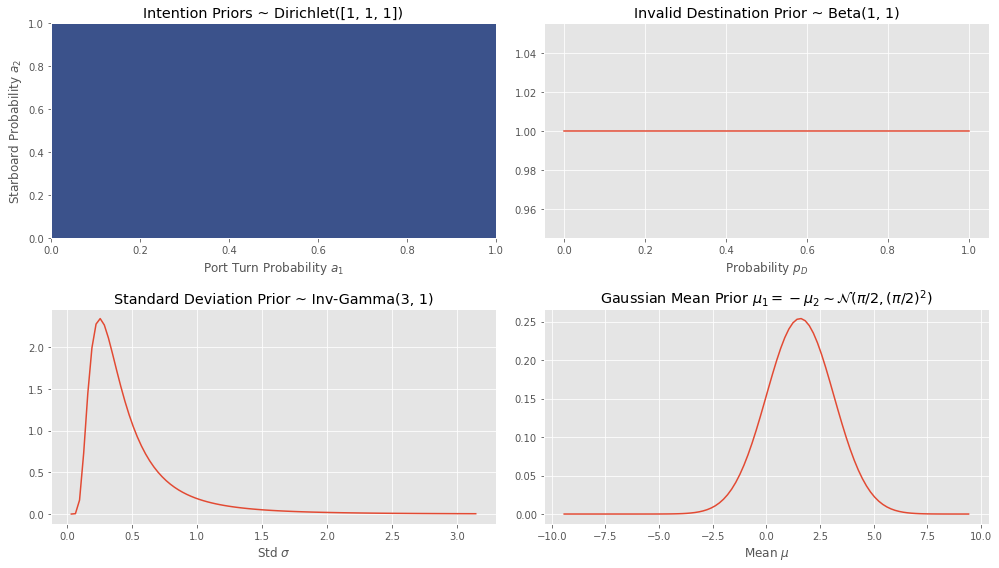
\includegraphics[width=1\textwidth]{figures/priors.png}
    \caption{Model priors for $\boldsymbol{\alpha}$, $p_D$, $\sigma$ and $\boldsymbol{\mu}$. The contour plot for $\boldsymbol{\alpha}$ shows $\alpha_1$ and $\alpha_2$, but $\alpha_0$ is implicitly included by the constraint $\alpha_0 = 1 - \alpha_1 - \alpha_2$. The priors for $\boldsymbol{\alpha}$ and $p_D$ are non-informative priors, while the priors for $\mu_2 = -\mu_1$ and $\sigma$ are informative priors selected by intuitive reasoning.}
    \label{fig:priors}
\end{figure}

The purpose of this chapter is to learn as much about the parameters $\boldsymbol{\alpha}$, $\mu$, $\sigma$ and $p_D$ from available observations $\mathcal{D}$, in this case only the angles $\mathcal{D} = \boldsymbol{\theta}$ are known. 

\section{Implementation}
Both \acrshort{mcmc} and \acrshort{vi} were implemented using Tensorflow Probability, as it has great support for both methods as well as it utilizes Tensorflows automatic differentiation to avoid dealing with error-prone calculations \cite{tensorflow2015-whitepaper}. The joint distribution in \cref{eq:example_joint} was implemented using the \texttt{JointDistributionSequential} distribution in TFP. (TODO: Add code in appendix)


\section{Dataset \& Benchmark}
The dataset was generated from $N=1000$ samples $\mathcal{D}$ from \cref{eq:angle_complete_mixture} with fixed parameters. A successful inference should be able to regain the parameters $\boldsymbol{\alpha}$, $p_D$, $\mu$ and $\sigma$ from $\mathcal{D}$.

\section{Markov Chain Monte Carlo}
Hamiltonian Monte Carlo was implemented using Tensorflow Probability (TFP). The log posterior target density was then defined using \cref{eq:example_unnormalized_posterior} as 
\begin{align}\label{eq:example_ll}
\begin{split}
    ll &= \log \tilde{p}(\boldsymbol{\mu}, \sigma, p_D, \boldsymbol{\alpha})
\end{split}
\end{align}


The proposal distribution were transformed using the following transformations (Bijectors)

\begin{itemize}
\item Softmax \eqref{eq:softmax} to unconstrain sampling of $\{\boldsymbol{\alpha} \in (0, 1)^3\ | \sum x_i = 1\}$
\item Sigmoid \eqref{eq:sigmoid} to unconstrain sampling of $p_D \in (0, 1)$
\item Softplus \eqref{eq:softplus} to unconstrain sampling of $\sigma > 0$
\item Softplus \eqref{eq:softplus} to acheive unimodal sampling of $\mu > 0$
\end{itemize}

$20$ individual chains were randomly initialized by sampling from the prior. $10000$ samples were then drawn from each chain, were the first $5000$ samples are discarded due to burn-in. These values were selected by trial and error, and by inspecting the individual chains in order to confirm convergence.  

\section{Variational Inference}

\acrshort{vi} was implemented using an independent, transformed Gaussian distribution as surrogate density for each variable. Specifying this model was easily achieved by passing the following list of Bijectors to \texttt{tfp.experimental.vi.build\_factored\_surrogate\_posterior}.
\begin{itemize}
\item Softmax \eqref{eq:softmax} to transform $\mathcal{R}^3$ to $\{\boldsymbol{\alpha} \in (0, 1)^3\ | \sum x_i = 1\}$
\item Sigmoid \eqref{eq:sigmoid} to transform $\mathcal{R}$ to $p_D \in (0, 1)$
\item Softplus \eqref{eq:softplus} to transform $\mathcal{R}$ to $\sigma > 0$
\item Softplus \eqref{eq:softplus} to achieve unimodal distribution of $\mu \in \mathcal{R}$
\end{itemize}

The last Softplus Bijector is especially important for \acrshort{vi} and deserves further explanation. As the intention probabilities for $I=1$ and $I=2$ are symmetrical around $\theta=0$ and the Gaussian distribution offer support on the entire real line $\mathcal{R}$, the resulting marginal distribution for $\mu$ becomes bimodal. As the model is not identifiable from $\boldsymbol{\theta}$ alone, the data supports both modes. The prior do prioritize the positive values, but still offers support for negative values as well.  Using \acrshort{vi} with reverse \acrshort{kl} may therefore result in fitting the wrong mode, as discussed in \cref{sec:im-mode}, unless $\mu > 0$ is explicitly enforced by using a Softplus transformation to remove support for negative values. 

The Stochastic Gradient Descent (SGD) optimizer \texttt{tf.optimizers.Adam} was then used to optimize the reverse KL divergence by passing it to \texttt{tfp.vi.fit\_surrogate\_posterior} along with the same log posterior density used for \acrshort{mcmc}, expressed in \cref{eq:example_ll} \cite{tensorflow2015-whitepaper}. 

\section{Results}
A dataset of $N=1000$ samples were used to observe how well \acrshort{vi} and \acrshort{mcmc} are able to learn from data. The true parameters used to generate the datasets are summarized in \cref{tbl:example_params}. The parameters were selected such that the priors are reasonable, while also making sure that the true parameters are different from the prior max and mean to verify that the values are actually learned from data. 
\begin{table}[h]
\centering
\begin{tabular}{lllll}
\textbf{Variable:}   & $\boldsymbol{\alpha}$ & $p_D$ & $\mu$                  & $\sigma$         \\ \hline
\textbf{Value:} & $[0.5, 0.3, 0.2]$     & $0.3$ & $\frac{\pi}{3}$ & $0.6$ \\
\end{tabular}
\caption{True values used to generate the dataset for example case 1.}
\label{tbl:example_params}
\end{table}


The posterior distribution when using \acrshort{mcmc} is shown in \cref{fig:example_mcmc_posterior} and shows how it is able to infer the intention probabilities $\boldsymbol{\alpha}$ from data, with the MAP estimates being pretty much spot-on. The uncertainty for the different intentions are however rather high, as multiple combinations of parameter values are able to explain the data rather well. The probability of invalid destination $p_D$ is also successfully reconstructed from observations, with rather low uncertainty. However, it it unable to distinguish between the mean $\mu$ and the standard deviation $\sigma$, resulting in high uncertainty and incorrect MAP estimates. The sampling took over 8 minutes in total for this dataset. 

\cref{fig:example_vi_posterior} show the performance of  \acrshort{vi} on the same dataset. The intention MAP values are close to the true parameters, though \acrshort{vi} severely underestimate the true uncertainty. For the invalid destination probability, the results are however much better with very similar results as \acrshort{mcmc}. For the mean $\mu$ and standard deviation $\sigma$, the results are comparable to \acrshort{mcmc}, though with less uncertainty. However, considering the optimization only used 22 seconds on the same computer, these results are quite impressive when compared to \acrshort{mcmc}.

Another dataset with only $N=50$ samples was generated to see how the methods behave will low amounts of data. \cref{fig:example_mcmc_vi_low_N} show how \acrshort{vi} is a bit overconfident on the intention probabilities and underestimate the uncertainty when compared to \acrshort{mcmc}. The results are otherwise very similar as shown in \cref{fig:example_mcmc_low_N} and \cref{fig:example_vi_low_N} for \acrshort{mcmc} and \acrshort{vi} respectively. Both methods are able to express the high uncertainty due to the limited amount of data available. 

Other datasets created with different parameters were also tested, though the plots are not included. Other datasets showed very similar results, only varying a bit on which variables the methods were able to correctly estimate. Random variations when generating the dataset also affected the final results, where some realizations of the data performed well and other performed poorly even if the parameters remained constant. 

The number of burn-in samples were somewhat arbitrarily chosen. However, by inspecting the individual chains in \cref{fig:example_mcmc_trace}, the individual chains appear to have reached the same stationary distribution and $5000$ burn-in samples are assumed to be enough for this specific problem.

\begin{figure}[h]
    \centering
    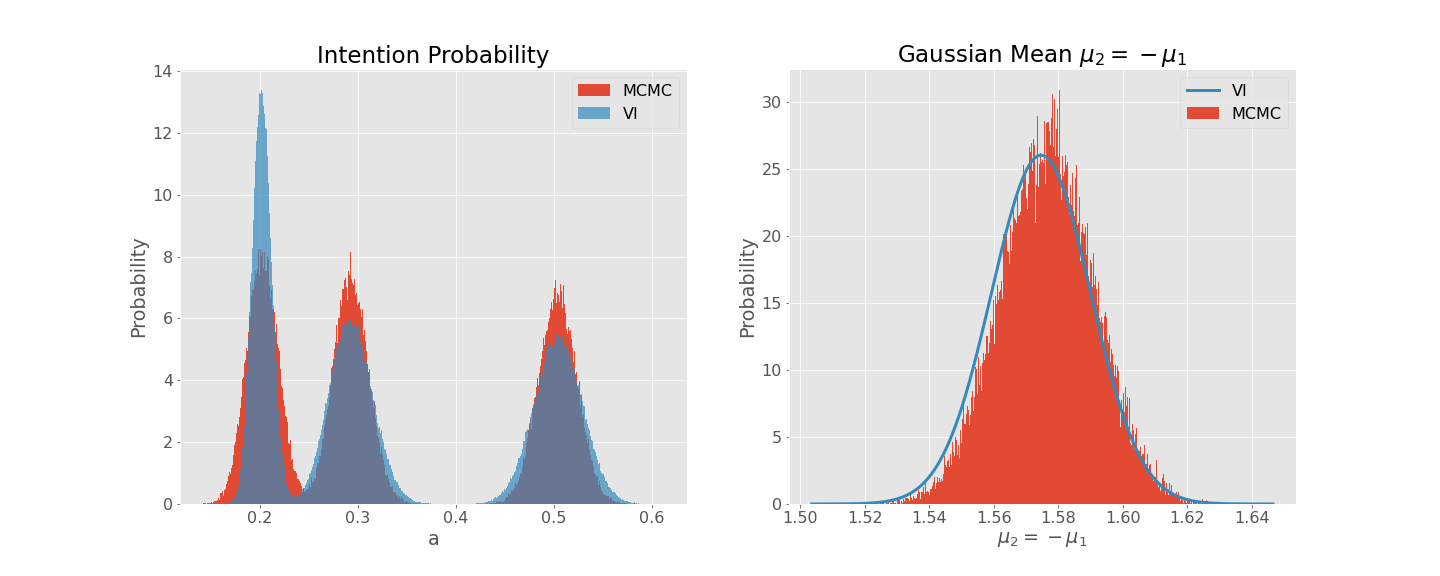
\includegraphics[width=\textwidth]{figures/example_vi_mcmc_comparison.png}
    \caption{The posterior distribution for intention probabilities and Gaussian mixture component means, found using MCMC and VI and plotted together to show how the methods give very comparable results. Note that all three intention probabilities are plotted together with the same color to highlight the differences between MCMC and VI. The plot shows how \acrshort{vi} underestimate the uncertainty when compared to \acrshort{mcmc}.}
    \label{fig:example_mcmc_vi_alphas}
\end{figure}

\begin{figure}[h]
    \centering
    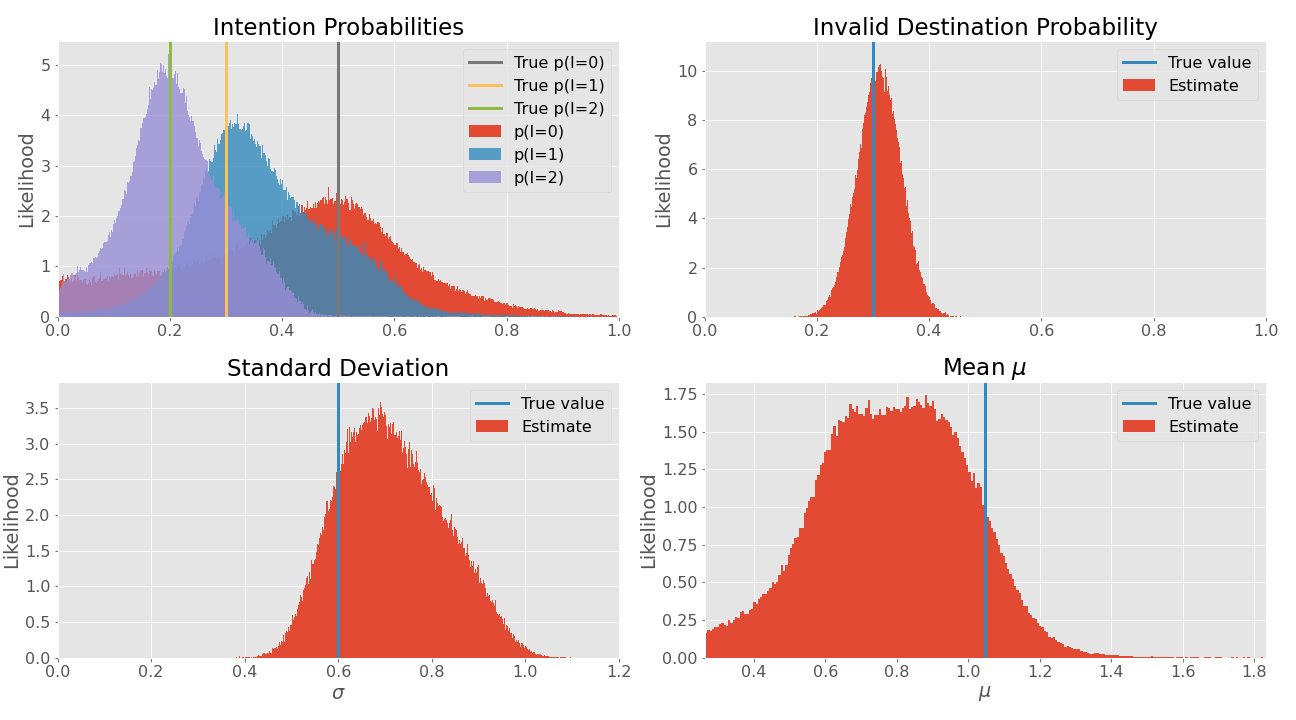
\includegraphics[width=\textwidth]{figures/example_mcmc.png}
    \caption{The posterior distribution for all variables using MCMC. The method is able to estimate the parameters from available data, though with rather high uncertainty. The MAP estimates are close to the true values for all parameters.}
    \label{fig:example_mcmc_posterior}
\end{figure}


\begin{figure}[h]
    \centering
    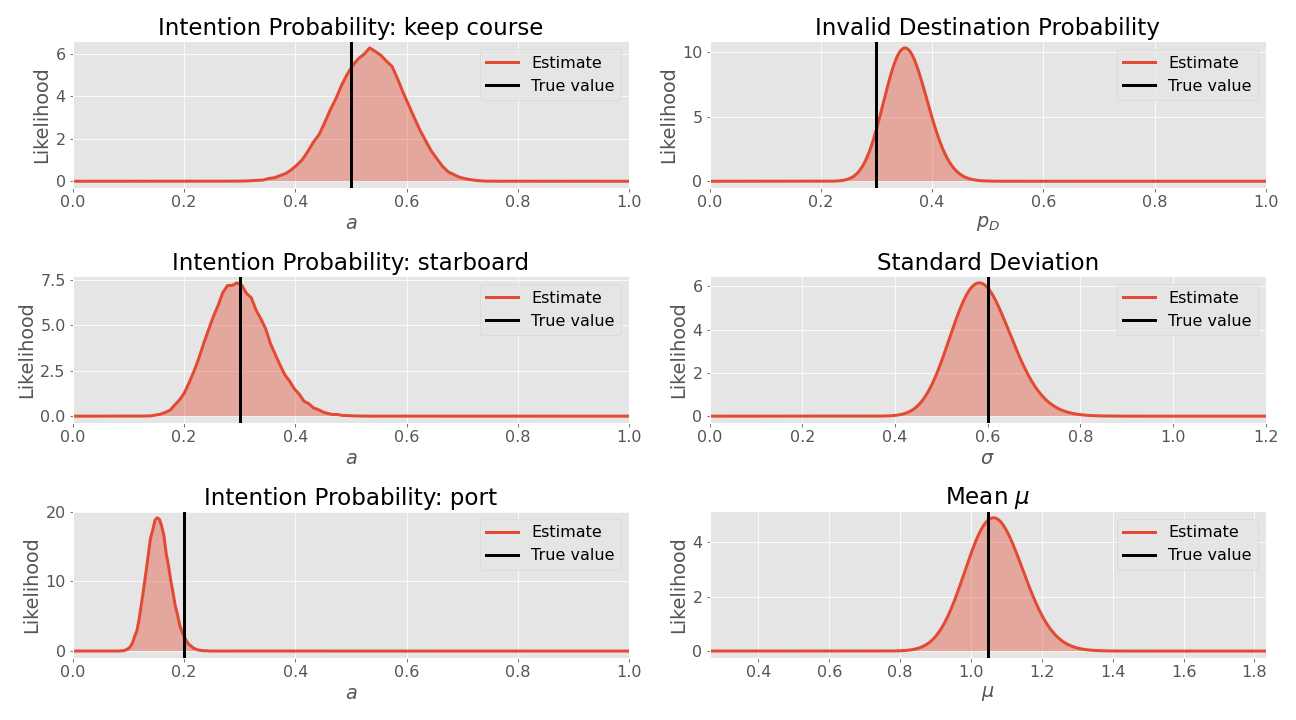
\includegraphics[width=\textwidth]{figures/example_vi.png}
    \caption{The posterior distribution for all variables using VI. The results are comparable to \acrshort{mcmc}, with very similar MAP estimates. The low uncertainty are however indicating overconfidence, especially when compared to \acrshort{mcmc}.}
    \label{fig:example_vi_posterior}
\end{figure}


\begin{figure}[h]
    \centering
    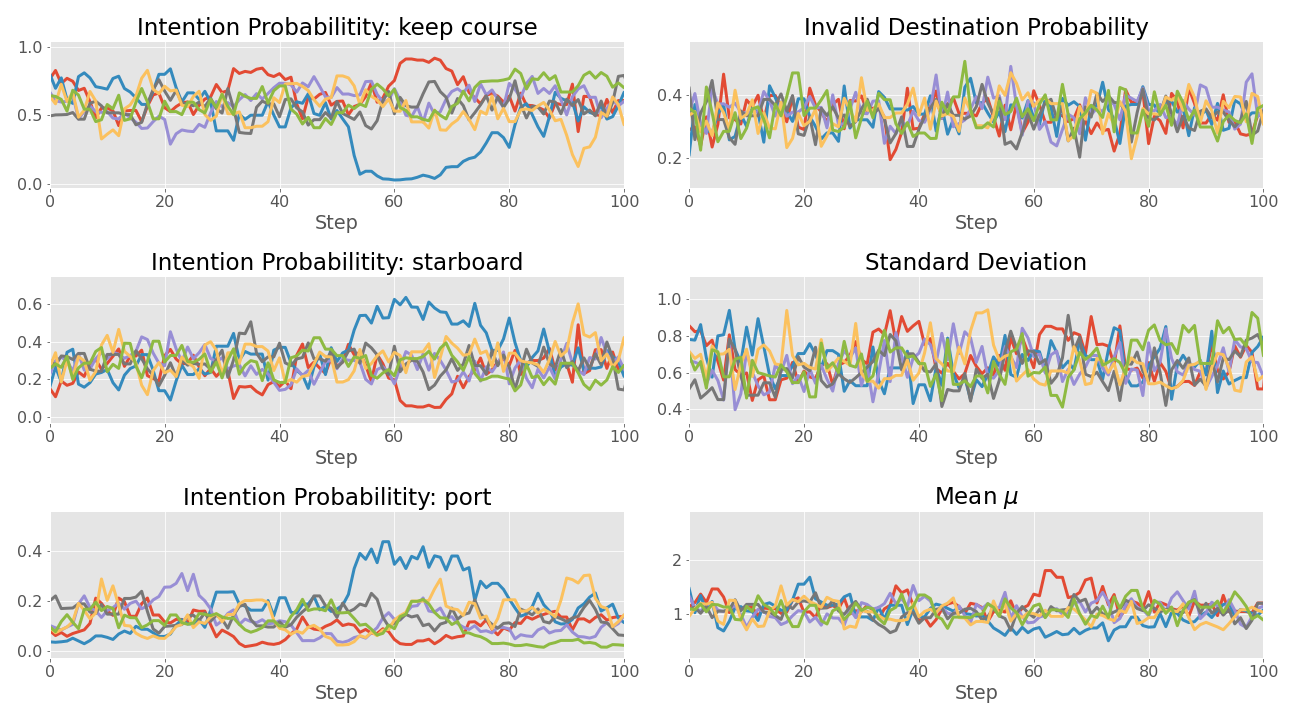
\includegraphics[width=\textwidth]{figures/example_mcmc_trace.png}
    \caption{Traceplot of the different chains. The chains appear to have reached a stationary distribution, and the current burn-in period of $5000$ samples are likely sufficient for this problem.}
    \label{fig:example_mcmc_trace}
\end{figure}

\begin{figure}[h]
    \centering
    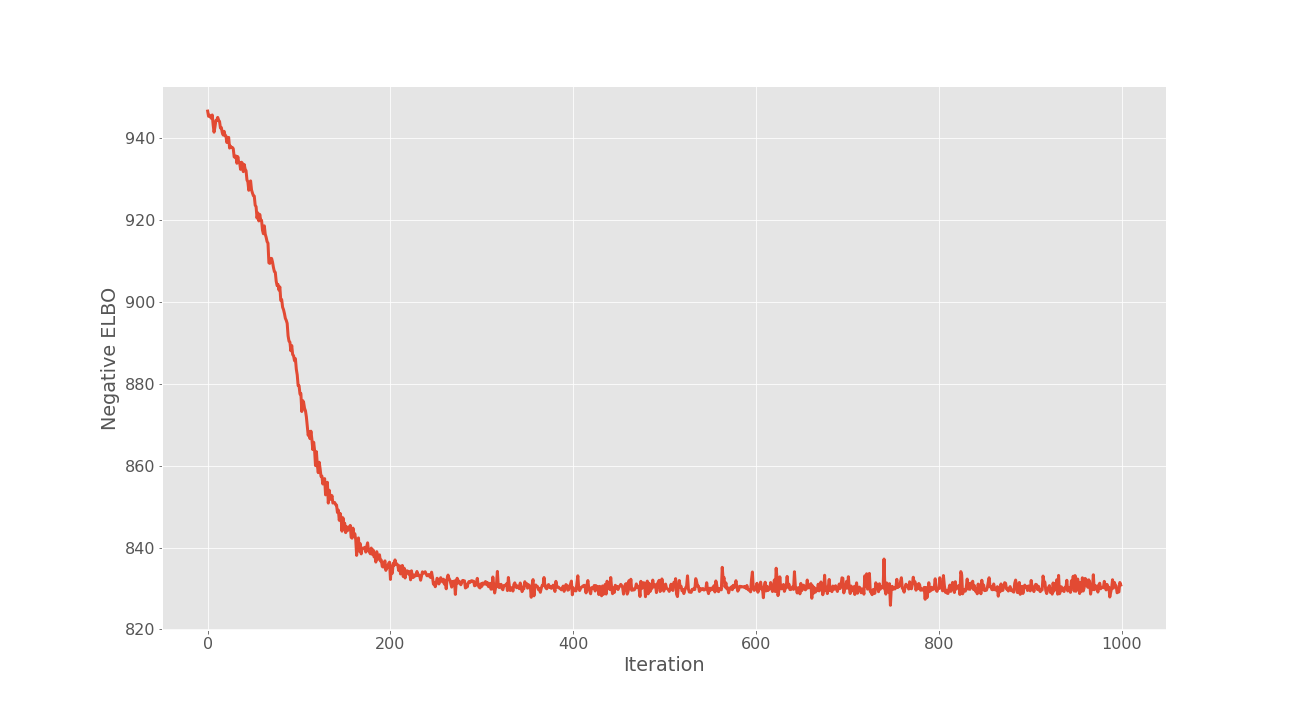
\includegraphics[width=\textwidth]{figures/example_vi_losses.png}
    \caption{Negative ELBO plotted against the fixed number of optimization steps for \acrshort{vi}. It reaches an optimum after less than $500$ steps and could in this case be stopped early to shorten the runtime.}
    \label{fig:example_vi_losses}
\end{figure}


\begin{figure}[h]
    \centering
    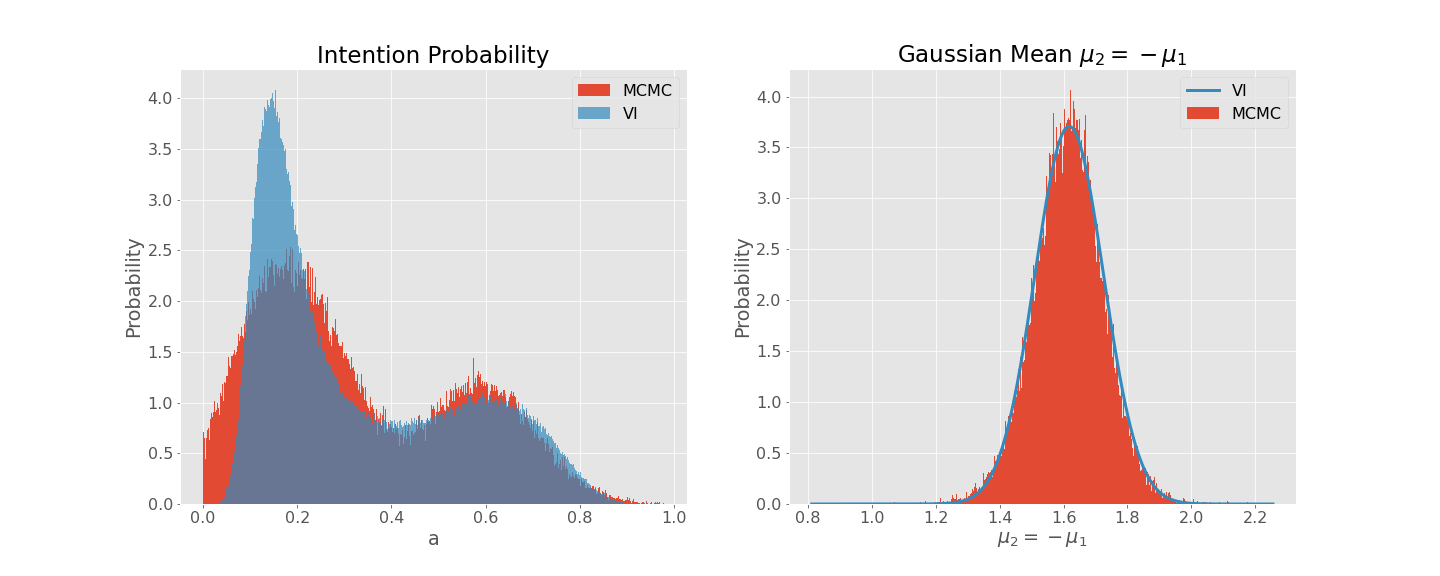
\includegraphics[width=\textwidth]{figures/example_vi_mcmc_comparison_low_N.png}
    \caption{Comparison of MCMC and VI for the parameters $\boldsymbol{\alpha}$ and $\mu$ with only $N=50$ samples. Both methods are able to express uncertainty due to low amount of data.}
    \label{fig:example_mcmc_vi_low_N}
\end{figure}

\begin{figure}[h]
    \centering
    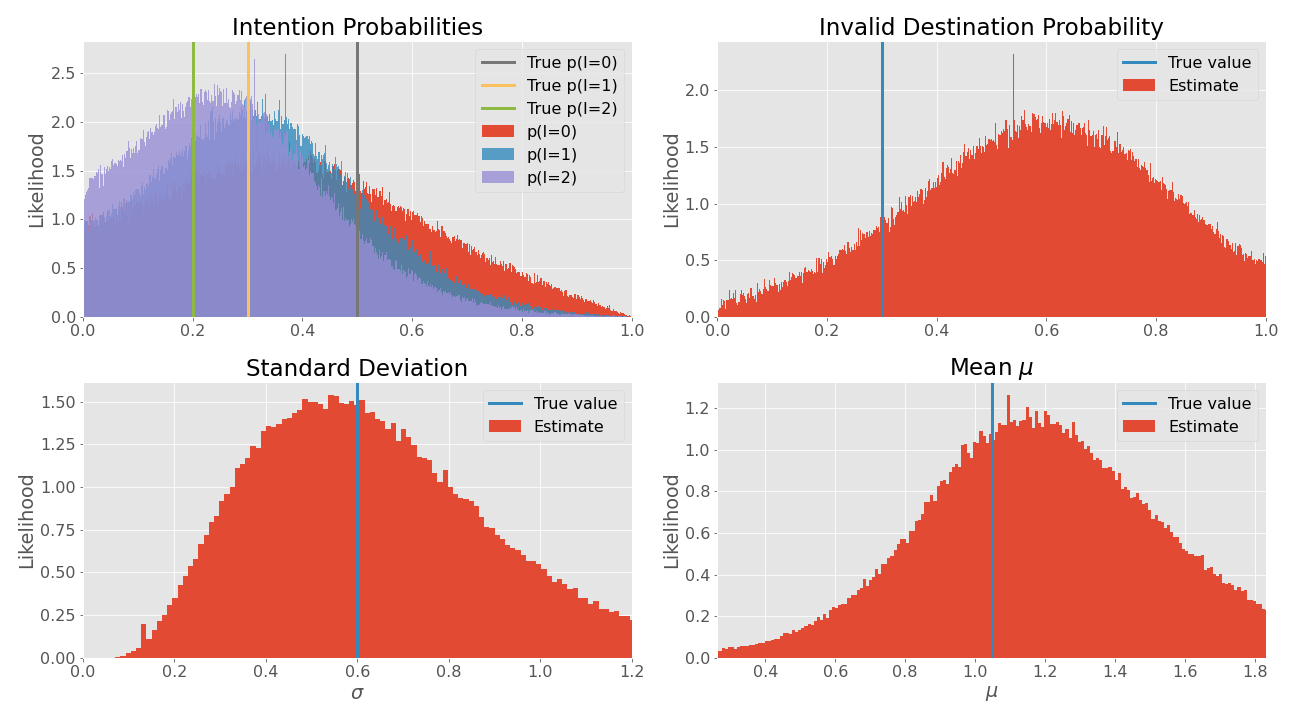
\includegraphics[width=\textwidth]{figures/example_mcmc_low_N.png}
    \caption{Posterior distribution approximated using \acrshort{mcmc} with only $N=50$ samples. The results shows large uncertainty for all parameters.}
    \label{fig:example_mcmc_low_N}
\end{figure}

\begin{figure}[h]
    \centering
    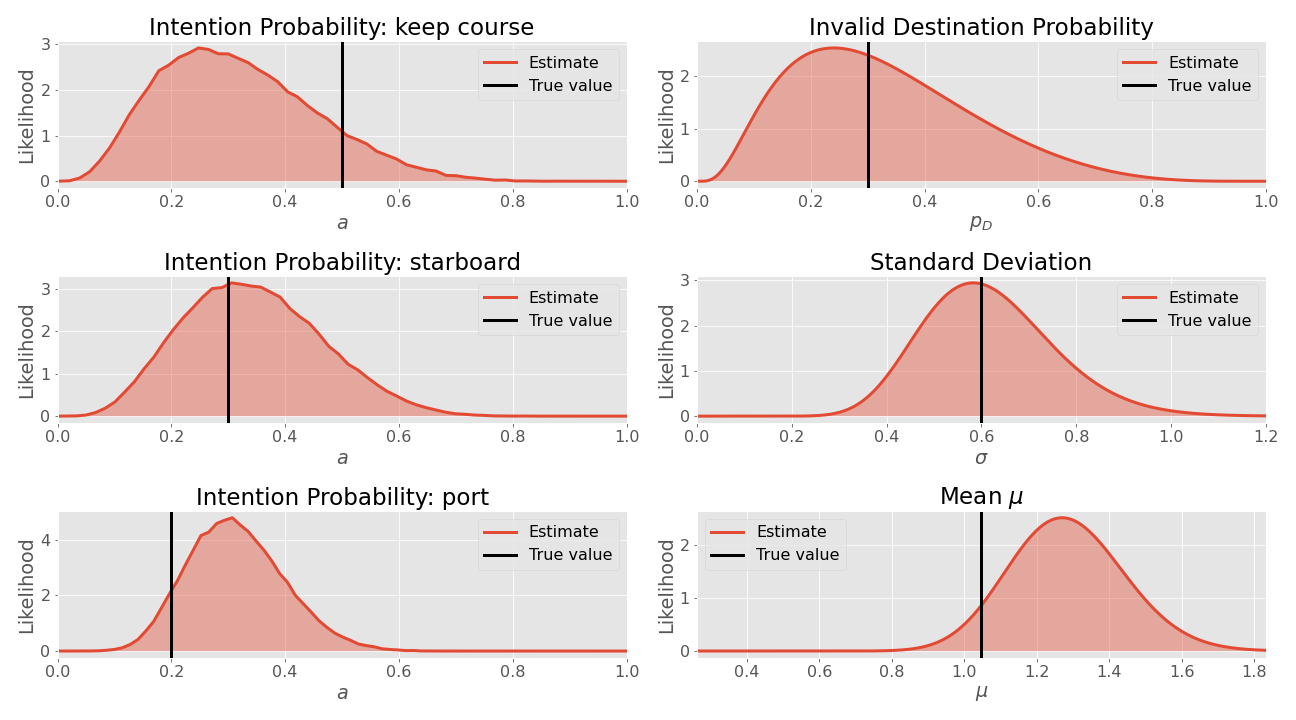
\includegraphics[width=\textwidth]{figures/example_vi_low_N.png}
    \caption{Posterior distribution approximated using \acrshort{vi} with only $N=50$ samples. The results shows large uncertainty for all parameters.}
    \label{fig:example_vi_low_N}
\end{figure}



\chapter{Discussion}

All of the methods described in this thesis so far have their strong advantages and disadvantages. 

\section{When all variables are discrete}
In the case of \acrshort{pgm}'s with only discrete variables, exact inference methods are often applicable. The challenges of Bayesian inference in such networks usually boils down to computational complexity when the number of variables increases. Exact methods such as \acrshort{bp} are in most cases the most appropriate choice, though some structures (in the case of loops) cannot guarantee an optimal solution. 

\section{When some variables are continuous}
When some variables are continuous, the problem usually gets a bit more complicated. If all parent-child can be expressed using conjugate-priors, exact methods can still be used. However, requiring the use of only conjugate-priors may in many cases be too restrictive as it limits the ability to express intuitive understanding of the data-generating process. 

The most straight-forward approach will be to use \acrshort{mcmc} methods, due to their simplicity. These methods allow sampling from arbitrarily complex models as long as the target probability can be evaluated. It can in most cases provide asymptotic guarantees that the samples is from the true posterior distribution, though only given a very large amount of samples. How many samples that are considered "enough" is difficult to say, and it usually require manual interpretations of the results in order to verify convergence. Using \acrshort{mcmc} in autonomous systems may therefore be challenging unless the model is sufficiently simple, in which case other methods may still be preferable. Due to the random nature of sampling methods, \acrshort{mcmc} is likely a poor choice for problems where deterministic behaviour is valued.



Though it requires more work, \acrshort{vi} will in many cases be a better option. By posing the problem as a optimization problem rather than relying on sampling, variational inference can give deterministic behaviour as well as drastically speed up inference when compared to \acrshort{mcmc}. However, \acrshort{vi} requires manual selection of a good surrogate density, and the choice of a bad surrogate may lead to poor results due to invalid assumptions. \acrshort{vi} does therefore by itself not provide any guarantees on the correctness of the results as it will always be limited by the assumptions and approximations used by the surrogate density.

A lot of research is currently focusing on how to apply \acrshort{vi} on more complicated models without the need of error-prone calculations or strict assumption. Methods such as variational message passing allows for more complicated surrogate densities in order to retain the interaction between variables in the model \cite{winnbishop}. 

In practice, both methods are likely needed. \acrshort{mcmc} methods can be used to "blindly" sample from the true posterior in order to aid the selection of a proper surrogate density. \acrshort{vi} can then be used to approximate the true posterior without loosing information to invalid assumptions. 

\section{}


\chapter{Conclusion}

You definitely should use the \texttt{ntnuthesis} \LaTeX{} document class for your thesis.


\chapter*{\bibname}
\printbibliography[heading=none]

\appendix
\chapter{Additional Material}
\label{app:additional}

%Additional material that does not fit in the main thesis but may still be relevant to share, e.g., raw data from experiments and surveys, code listings, additional plots, pre-project reports, project agreements, contracts, logs etc., can be put in appendices. Simply issue the command \texttt{\textbackslash appendix} in the main \texttt{.tex} file, and make one chapter per appendix.

%If the appendix is in the form of a ready-made PDF file, it should be supported by a small descriptive text, and included using the \texttt{pdfpages} package. To illustrate how it works, a standard project agreement (for the IE faculty at NTNU in Gjøvik) is attached here. You would probably want the included PDF file to begin on an odd (right hand) page, which is achieved by using the \texttt{\textbackslash cleardoublepage} command immediately before the \texttt{\textbackslash includepdf[]\{\}} command. Use the option \texttt{[pages=-]} to include all pages of the PDF document, or, e.g., \texttt{[pages=2-4]} to include only the given page range.

\cleardoublepage
%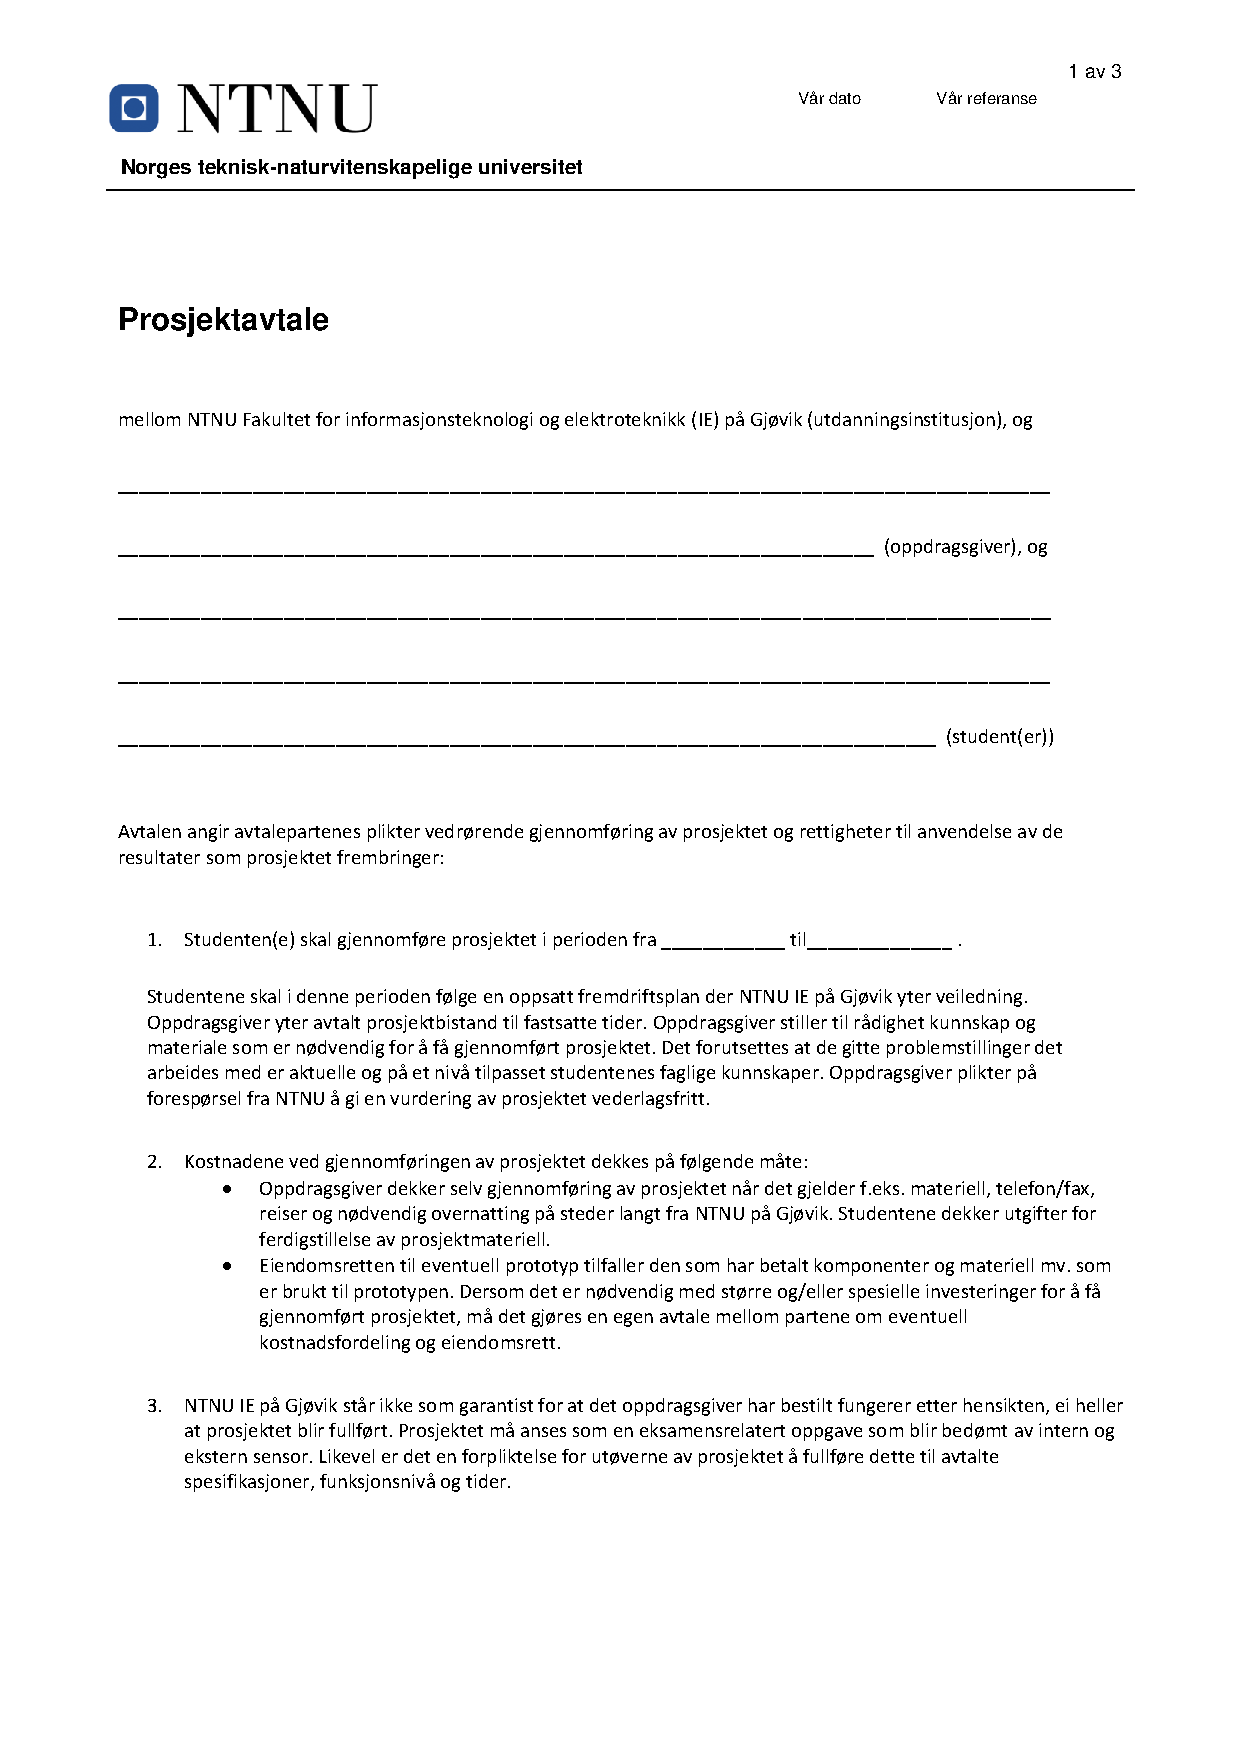
\includepdf[pages=-]{appendices/NTNUProsjektavtale.pdf}

\end{document}
